% =============================================================================
%  Machine Learning for Petroleum Engineers Using Python
%  Clase 3: pandas y Carga de Datos --- Producción y Well Logs (Volve)
%  SLB Ecuador | UDLA
%
%  Compilar: pdflatex -shell-escape presentacion.tex (x2 para refs)
% =============================================================================
\documentclass[aspectratio=169, 11pt]{beamer}

% ── Codificación y lenguaje ──────────────────────────────────────────────────
\usepackage[T1]{fontenc}
\usepackage[utf8]{inputenc}
\usepackage[spanish,es-noshorthands]{babel}

% ── Fuentes ──────────────────────────────────────────────────────────────────
\usepackage{FiraSans}
\usepackage{FiraMono}
\renewcommand{\familydefault}{\sfdefault}

% ── Gráficos y diagramas ────────────────────────────────────────────────────
\usepackage{graphicx}
\usepackage{tikz}
\usetikzlibrary{arrows.meta, positioning, shapes.geometric, calc, fit, decorations.pathreplacing}
\usepackage{fontawesome5}

% ── Código fuente ────────────────────────────────────────────────────────────
\usepackage{minted}
\usepackage{tcolorbox}
\tcbuselibrary{minted, skins, breakable}

% ── Tablas y utilidades ──────────────────────────────────────────────────────
\usepackage{amsmath}
\usepackage{colortbl}
\usepackage{booktabs}
\usepackage{multicol}
\usepackage{hyperref}
\usepackage{calc}

% =============================================================================
%  PALETA DE COLORES (rojo UDLA + variantes)
% =============================================================================
\definecolor{arcaRed}{HTML}{C82B40}
\definecolor{arcaDark}{HTML}{6B1525}
\definecolor{udlaCrimson}{HTML}{A31545}
\definecolor{arcaGray}{HTML}{F5F5F5}
\definecolor{arcaLightGray}{HTML}{EBEBEB}
\definecolor{textDark}{HTML}{2D2D2D}
\definecolor{textMuted}{HTML}{6B7280}
\definecolor{codeGreen}{HTML}{16A34A}
\definecolor{codeBlue}{HTML}{2563EB}
\definecolor{codeOrange}{HTML}{EA580C}
\definecolor{slbBlue}{HTML}{0014DC}
\definecolor{terminalBg}{HTML}{0F172A}
\definecolor{terminalGreen}{HTML}{86EFAC}
\definecolor{terminalMuted}{HTML}{94A3B8}
\definecolor{codeBg}{HTML}{FAFAFA}

% =============================================================================
%  CONFIGURACIÓN DEL TEMA BEAMER
% =============================================================================
\usetheme{default}
\usecolortheme{default}

\setbeamertemplate{navigation symbols}{}
\setbeamertemplate{footline}{}
\setbeamertemplate{headline}{}

\setbeamercolor{normal text}{fg=textDark}
\setbeamercolor{frametitle}{fg=arcaRed, bg=white}
\setbeamercolor{title}{fg=white}
\setbeamercolor{subtitle}{fg=white!85}
\setbeamercolor{author}{fg=white!80}
\setbeamercolor{date}{fg=white!70}
\setbeamercolor{item}{fg=arcaRed}
\setbeamercolor{subitem}{fg=arcaDark}
\setbeamercolor{block title}{fg=white, bg=arcaRed}
\setbeamercolor{block body}{fg=textDark, bg=arcaGray}
\setbeamercolor{block title alerted}{fg=white, bg=codeOrange}
\setbeamercolor{block body alerted}{fg=textDark, bg=arcaGray}
\setbeamercolor{block title example}{fg=white, bg=codeGreen}
\setbeamercolor{block body example}{fg=textDark, bg=arcaGray}
\setbeamercolor{section in toc}{fg=arcaDark}

\setbeamerfont{frametitle}{size=\Large, series=\bfseries}
\setbeamerfont{title}{size=\huge, series=\bfseries}
\setbeamerfont{subtitle}{size=\large}
\setbeamerfont{author}{size=\normalsize}
\setbeamerfont{date}{size=\small}
\setbeamerfont{block title}{size=\normalsize, series=\bfseries}
\setbeamerfont{footnote}{size=\tiny}

\setbeamertemplate{itemize item}{\scriptsize\raise1.5pt\hbox{\color{arcaRed}$\blacktriangleright$}}
\setbeamertemplate{itemize subitem}{\scriptsize\raise1pt\hbox{\color{arcaDark}$\bullet$}}
\setbeamertemplate{enumerate items}[default]
\setbeamercolor{enumerate item}{fg=arcaRed}

% =============================================================================
%  HEADER
% =============================================================================
\setbeamertemplate{headline}{%
  \begin{tikzpicture}[remember picture, overlay]
    \fill[arcaDark] (current page.north west) rectangle
      ([yshift=-0.7cm]current page.north east);
    \node[anchor=west, inner sep=0pt] at
      ([xshift=0.6cm, yshift=-0.35cm]current page.north west)
      {
\includegraphics[height=0.45cm]{../logo_udla_white.png}};
    \node[anchor=east, inner sep=0pt] at
      ([xshift=-0.6cm, yshift=-0.35cm]current page.north east)
      {\includegraphics[height=0.42cm]{../SLB_white.png}};
  \end{tikzpicture}%
  \vspace{0.7cm}%
}

% =============================================================================
%  FOOTER
% =============================================================================
\setbeamertemplate{footline}{%
  \begin{tikzpicture}[remember picture, overlay]
    \draw[arcaLightGray, line width=0.4pt]
      ([yshift=0.55cm, xshift=0.6cm]current page.south west) --
      ([yshift=0.55cm, xshift=-0.6cm]current page.south east);
    \node[anchor=south, font=\tiny\color{textMuted}] at
      ([yshift=0.15cm]current page.south)
      {Machine Learning for Petroleum Engineers Using Python \(\cdot\) SLB Ecuador};
    \node[anchor=south east, font=\scriptsize\bfseries\color{arcaRed}] at
      ([xshift=-0.6cm, yshift=0.15cm]current page.south east)
      {\insertframenumber};
  \end{tikzpicture}%
}

% =============================================================================
%  FRAMETITLE personalizado con línea roja
% =============================================================================
\setbeamertemplate{frametitle}{%
  \vspace{0.25cm}%
  \usebeamerfont{frametitle}\usebeamercolor[fg]{frametitle}\insertframetitle%
  \par\vspace{2pt}%
  \begin{tikzpicture}
    \fill[arcaRed] (0,0) rectangle (3cm, 1.5pt);
    \fill[arcaLightGray] (3cm,0) rectangle (\textwidth, 0.5pt);
  \end{tikzpicture}%
  \vspace{0.1cm}%
}

% =============================================================================
%  ESTILO DE BLOQUES DE CÓDIGO (minted + tcolorbox)
% =============================================================================
\newtcblisting{pyblock}[1][]{%
  listing engine=minted,
  minted language=python,
  minted style=xcode,
  minted options={
    fontsize=\small,
    linenos=false,
    breaklines=true,
    python3=true
  },
  enhanced,
  colback=codeBg,
  colframe=arcaRed,
  left=8pt,
  right=6pt,
  top=5pt,
  bottom=5pt,
  boxrule=0pt,
  leftrule=3pt,
  arc=3pt,
  listing only,
  title={\hspace{-2pt}\faPython\hspace{5pt}Python},
  fonttitle=\scriptsize\bfseries,
  colbacktitle=arcaRed,
  coltitle=white,
  attach boxed title to top left={xshift=8pt, yshift=-7pt},
  boxed title style={
    arc=2pt, boxrule=0pt,
    top=1.5pt, bottom=1.5pt, left=6pt, right=6pt
  },
  drop fuzzy shadow=black!12,
  #1
}

\newtcblisting{outputblock}[1][]{%
  listing engine=minted,
  minted language=text,
  minted style=bw,
  minted options={
    fontsize=\small,
    breaklines=true,
    formatcom=\color{terminalGreen}
  },
  enhanced,
  colback=terminalBg,
  colframe=terminalBg,
  coltext=terminalGreen,
  left=10pt, right=6pt, top=5pt, bottom=5pt,
  boxrule=0pt,
  arc=3pt,
  listing only,
  title={\hspace{-2pt}\faTerminal\hspace{5pt}Output},
  fonttitle=\scriptsize\bfseries,
  colbacktitle=terminalGreen!85!black,
  coltitle=terminalBg,
  attach boxed title to top left={xshift=8pt, yshift=-7pt},
  boxed title style={
    arc=2pt, boxrule=0pt,
    top=1.5pt, bottom=1.5pt, left=6pt, right=6pt
  },
  #1
}

% =============================================================================
%  SECTION DIVIDERS
% =============================================================================
\newcommand{\sectionframe}[2]{%
  \begingroup
    \setbeamertemplate{headline}{}
    \setbeamertemplate{footline}{}
    \setbeamertemplate{navigation symbols}{}
    \begin{frame}[plain, noframenumbering]
      \begin{tikzpicture}[remember picture, overlay]
        \fill[arcaRed] (current page.south west) rectangle (current page.north east);
        \node[anchor=center, text=white, font=\Huge\bfseries, text width=12cm,
              align=center] at ([yshift=0.5cm]current page.center) {#1};
        \node[anchor=center, text=white!80, font=\large, text width=10cm,
              align=center] at ([yshift=-0.8cm]current page.center) {#2};
      \end{tikzpicture}
    \end{frame}
  \endgroup
}

% =============================================================================
%  METADATOS
% =============================================================================
\title{Machine Learning for Petroleum Engineers\\Using Python}
\subtitle{Módulo 3 · Clase 3: No Linealidad --- Árboles y Random Forest}
\author{Carlos Enrique Mosquera Trujillo}
\date{2026}

% =============================================================================
%  DOCUMENTO
% =============================================================================
% =============================================================================
%  DOCUMENTO
% =============================================================================
\begin{document}

% ── PORTADA ──────────────────────────────────────────────────────────────────
{
\setbeamertemplate{headline}{}
\setbeamertemplate{footline}{}
\begin{frame}[plain, noframenumbering]
  \begin{tikzpicture}[remember picture, overlay]
    \fill[white] (current page.south west) rectangle (current page.north east);
    \fill[arcaRed] (current page.north west) rectangle ([yshift=-0.35cm]current page.north east);
    \fill[arcaDark] (current page.south west) rectangle ([yshift=0.35cm]current page.south east);
    \fill[arcaRed]
      ([xshift=1.1cm, yshift=-0.35cm]current page.north west) rectangle
      ([xshift=1.15cm, yshift=0.35cm]current page.south west);
    \node[anchor=north west, inner sep=0pt] at
      ([xshift=1.8cm, yshift=-1.2cm]current page.north west)
      {
\includegraphics[height=1.6cm]{../logo_udla.png}};
    \node[anchor=north east, inner sep=0pt] at
      ([xshift=-1.5cm, yshift=-1.2cm]current page.north east)
      {\includegraphics[height=1.5cm]{../SLB.png}};
    \node[anchor=center, text=arcaDark, text width=14.5cm, align=center] at
      ([yshift=0.95cm]current page.center) {
        {\LARGE\bfseries Machine Learning for Petroleum Engineers}\\[8pt]
        {\LARGE\bfseries Using Python}
      };
    \fill[arcaRed]
      ([yshift=-0.35cm, xshift=-3.2cm]current page.center) rectangle
      ([yshift=-0.28cm, xshift=3.2cm]current page.center);
    \node[anchor=center, text=arcaRed, font=\large, text width=13cm, align=center] at
      ([yshift=-1.3cm]current page.center) {
        Módulo 3 · Clase 3\\[3pt]
        No Linealidad: Árboles de Decisión y Random Forest
      };
    \node[anchor=center, text=textMuted, font=\normalsize] at
      ([yshift=-2.5cm]current page.center) {
        {\color{arcaRed}\faUser}\hspace{6pt}Carlos Enrique Mosquera Trujillo
        \hspace{16pt}
        {\color{arcaRed}\faIndustry}\hspace{4pt}SLB Ecuador
      };
  \end{tikzpicture}
\end{frame}
}

% ── ABRIR CON EL PROBLEMA ────────────────────────────────────────────────────
\begin{frame}{El Problema: la Realidad no Está Obligada a Ser una Recta}
  \vspace{-6pt}
  {\small\color{arcaDark}\bfseries
    Hasta ahora usamos modelos lineales. Funcionan muy bien cuando el efecto es parejo. ¿Pero qué pasa cuando no lo es?}

  \vspace{6pt}
  \begin{columns}[T]
    \begin{column}{0.50\textwidth}
      {\footnotesize\color{textMuted}
      \begin{itemize}\setlength{\itemsep}{7pt}
        \item[{\color{arcaRed}\scriptsize\faOilCan}]
          Abrir el choke 10 puntos no siempre agrega el mismo caudal.
        \item[{\color{arcaRed}\scriptsize\faChartLine}]
          La producción cae rápido al inicio y lentamente después.
        \item[{\color{arcaRed}\scriptsize\faThermometerHalf}]
          Temperatura y viscosidad tienen una relación exponencial.
        \item[{\color{arcaRed}\scriptsize\faProjectDiagram}]
          Una clase puede envolver a otra: no existe una línea que las separe.
      \end{itemize}}
    \end{column}
    \begin{column}{0.46\textwidth}
      \begin{tcolorbox}[colback=arcaGray,colframe=arcaRed,boxrule=0pt,
        leftrule=3pt,arc=3pt,left=7pt,right=7pt,top=7pt,bottom=7pt]
        {\small\color{arcaDark}\bfseries La pregunta de la clase}\\[5pt]
        {\footnotesize\color{textMuted}
          ¿Cómo construimos modelos capaces de reconocer
          \textbf{curvas, umbrales e interacciones}, sin tener que
          escribir de antemano la ecuación física exacta?}
      \end{tcolorbox}
      \vspace{7pt}
      {\scriptsize\color{arcaDark}\itshape
        Hoy veremos la misma solución en dos decisiones:
        estimar un número y predecir una clase.}
    \end{column}
  \end{columns}
\end{frame}

\begin{frame}[shrink=5]{Cuatro Formas que una Recta no Puede Representar Bien}
  \vspace{-6pt}
  \centering
  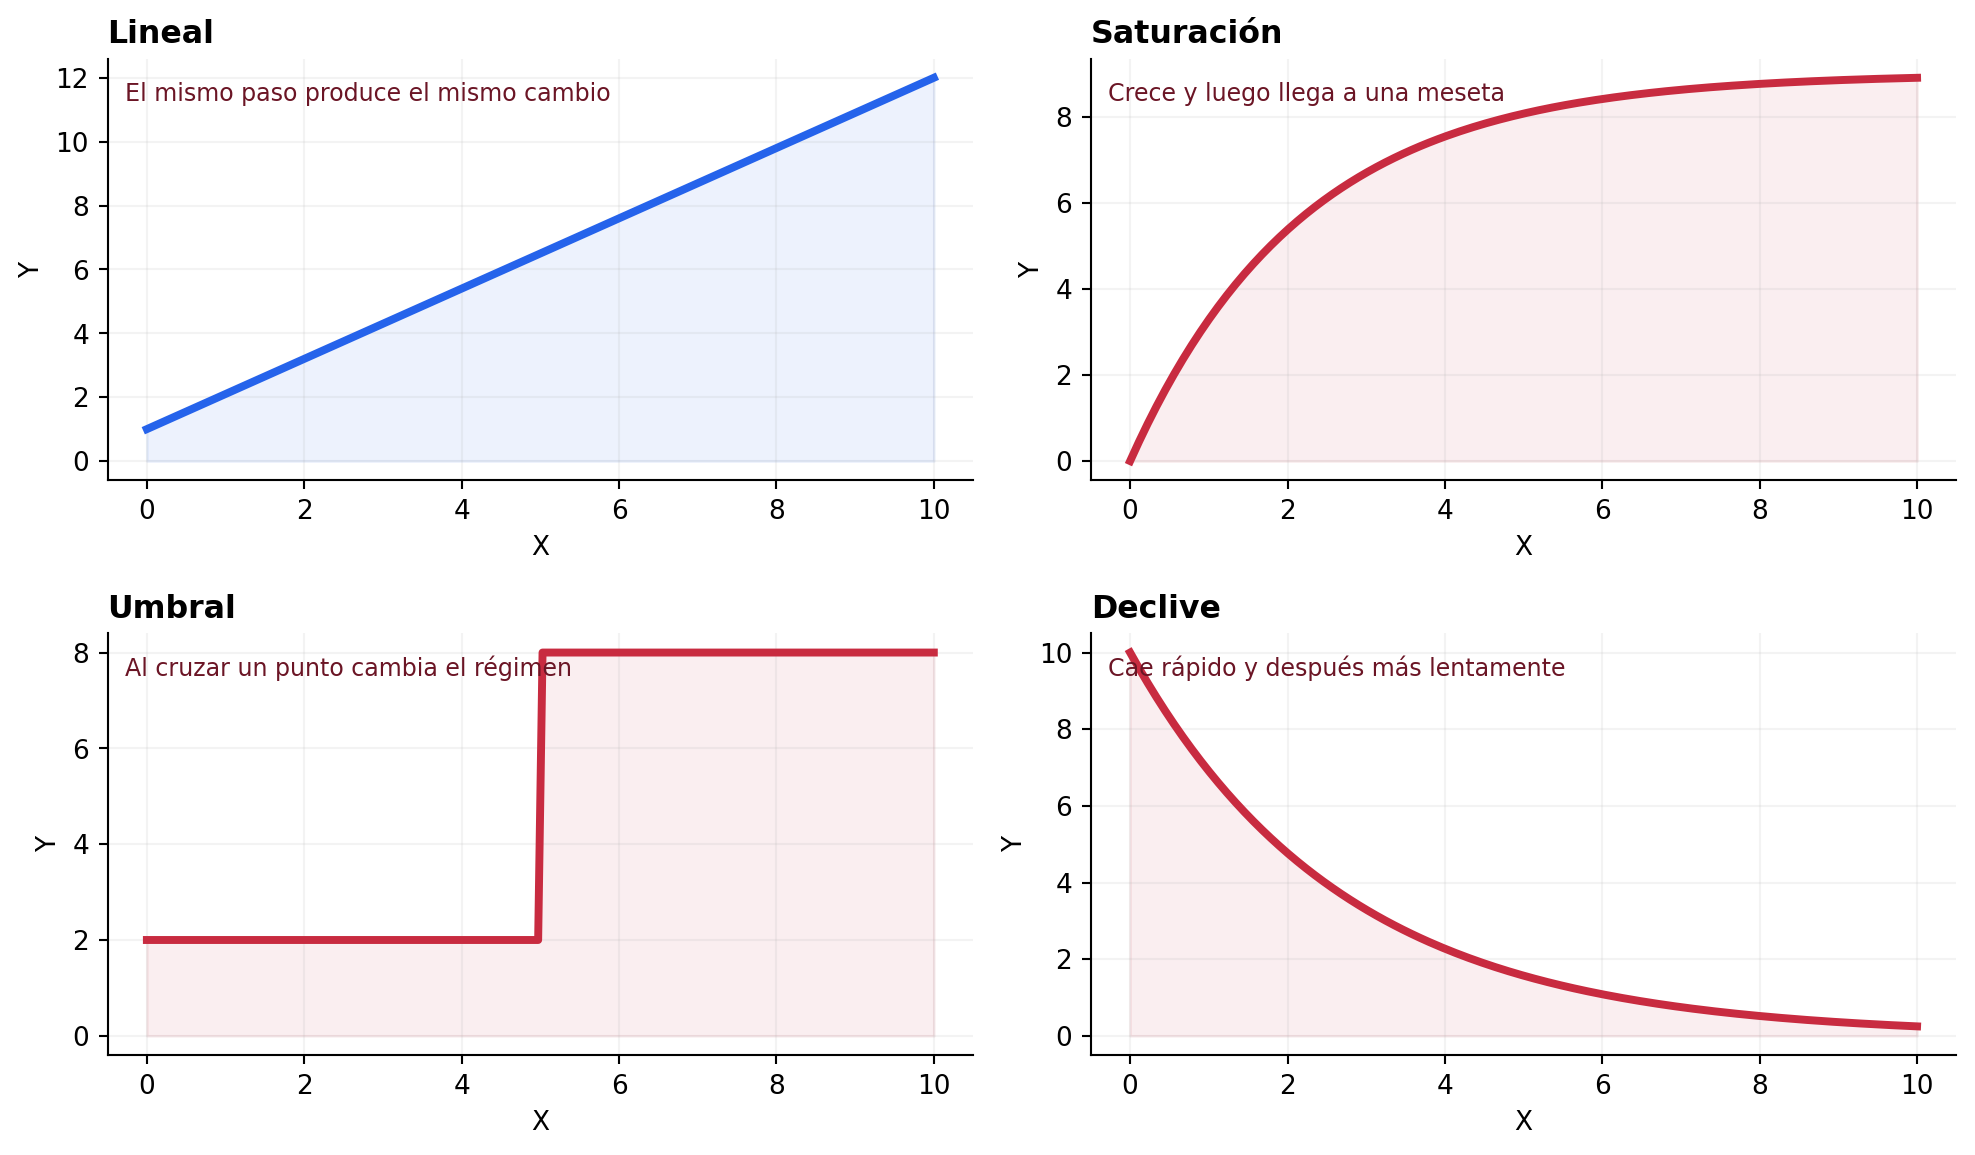
\includegraphics[width=0.88\textwidth,height=0.66\textheight,keepaspectratio]{fig_galeria_nolineal.png}

  \vspace{2pt}
  {\footnotesize\color{textMuted}
    La no linealidad no significa ``caos'': significa que el cambio
    \textbf{depende de dónde estamos}, puede saturarse o cambiar de régimen.}
\end{frame}

\begin{frame}{El Límite no es Falta de Datos: es la Forma del Modelo}
  \vspace{-6pt}
  \begin{columns}[T]
    \begin{column}{0.47\textwidth}
      \begin{tcolorbox}[colback=arcaGray,colframe=arcaRed,boxrule=0pt,
        leftrule=3pt,arc=3pt,left=7pt,right=7pt,top=6pt,bottom=6pt]
        {\small\color{arcaRed}\bfseries Regresión lineal}\\[4pt]
        {\footnotesize\color{textMuted}
          Solo puede ajustar un plano:
          \[
            \hat y=\beta_0+\beta_1x_1+\cdots+\beta_px_p
          \]
          Cada variable conserva el mismo efecto en todo el rango.}
      \end{tcolorbox}
    \end{column}
    \begin{column}{0.47\textwidth}
      \begin{tcolorbox}[colback=arcaGray,colframe=codeBlue,boxrule=0pt,
        leftrule=3pt,arc=3pt,left=7pt,right=7pt,top=6pt,bottom=6pt]
        {\small\color{codeBlue}\bfseries Regresión logística}\\[4pt]
        {\footnotesize\color{textMuted}
          Convierte ese plano en probabilidad, pero su frontera
          de decisión sigue siendo \textbf{una línea o un plano}.\\[7pt]
          Cambia la salida; no cambia la geometría interna.}
      \end{tcolorbox}
    \end{column}
  \end{columns}
  \vspace{10pt}
  \centering
  {\small\color{arcaDark}\bfseries
    Si el patrón es curva, ninguna cantidad de entrenamiento hará que una recta se doble.}
\end{frame}

% ── RECAP + RUTA ─────────────────────────────────────────────────────────────
\begin{frame}{Dónde Estamos}
  \vspace{-6pt}
  \begin{columns}[T]
    \begin{column}{0.48\textwidth}
      {\small\color{arcaDark}\bfseries\faCheckCircle\hspace{5pt}Ya tenemos:}
      \vspace{4pt}
      {\footnotesize\color{textMuted}
      \begin{itemize}\setlength{\itemsep}{3pt}
        \item[{\color{codeGreen}\scriptsize\faCheck}]
          Regresión lineal: predecir un \textbf{número}
        \item[{\color{codeGreen}\scriptsize\faCheck}]
          Regresión logística: predecir una \textbf{etiqueta}
        \item[{\color{codeGreen}\scriptsize\faCheck}]
          Métricas + \textbf{costo de negocio} y umbral
        \item[{\color{codeGreen}\scriptsize\faCheck}]
          Train/test, estandarización, binarización
      \end{itemize}
      }
      \vspace{6pt}
      {\scriptsize\color{textMuted}\itshape
        Pero ambos modelos comparten un límite:
        por dentro son \textbf{una recta}.}
    \end{column}
    \begin{column}{0.48\textwidth}
      {\small\color{arcaDark}\bfseries\faForward\hspace{5pt}Hoy:}
      \vspace{4pt}
      {\footnotesize\color{textMuted}
      \begin{itemize}\setlength{\itemsep}{3pt}
        \item[{\color{arcaRed}\scriptsize\faArrowRight}]
          Qué es la \textbf{no linealidad} y por qué el mundo
          real casi siempre es así
        \item[{\color{arcaRed}\scriptsize\faArrowRight}]
          Ver a la recta \textbf{fracasar} (las lunas y un
          problema real)
        \item[{\color{arcaRed}\scriptsize\faArrowRight}]
          \textbf{Árboles de decisión}: cutoffs automatizados
        \item[{\color{arcaRed}\scriptsize\faStar}]
          \textbf{Random Forest}: la sabiduría de la multitud
      \end{itemize}
      }
      \vspace{4pt}
      {\scriptsize\color{arcaDark}\itshape
        Reto de hoy: un \textbf{medidor virtual de flujo}.}
    \end{column}
  \end{columns}
\end{frame}

% ═════════════════════════════════════════════════════════════════════════════
\sectionframe{¿Qué es la No Linealidad?}{Cuando el paso deja de ser parejo}
% ═════════════════════════════════════════════════════════════════════════════

% ── RECAP LINEAL / DEFINICIÓN ────────────────────────────────────────────────
\begin{frame}[shrink=5]{Recuerden: Lineal = el Paso Parejo}
  \vspace{-6pt}
  {\small\color{arcaDark}\bfseries
    En la Clase 1 lo definimos: lineal es cuando el mismo paso en X produce \textbf{siempre el mismo} paso en Y.}

  \vspace{8pt}
  \begin{columns}[T]
    \begin{column}{0.48\textwidth}
      \begin{tcolorbox}[colback=arcaGray, colframe=codeGreen, boxrule=0pt, leftrule=3pt,
        arc=3pt, left=6pt, right=6pt, top=5pt, bottom=5pt]
        {\scriptsize\color{codeGreen}\bfseries\faCheck\hspace{4pt}LINEAL (el paso vale igual)}\\[4pt]
        {\scriptsize\color{textMuted}
          Tanquear el carro: el galón 1 cuesta lo mismo
          que el galón 10.\\[3pt]
          Presión hidrostática: cada 100 m suman
          \(\approx\) lo mismo.}
      \end{tcolorbox}
    \end{column}
    \begin{column}{0.48\textwidth}
      \begin{tcolorbox}[colback=arcaGray, colframe=arcaRed, boxrule=0pt, leftrule=3pt,
        arc=3pt, left=6pt, right=6pt, top=5pt, bottom=5pt]
        {\scriptsize\color{arcaRed}\bfseries\faTimes\hspace{4pt}NO LINEAL (el paso cambia)}\\[4pt]
        {\scriptsize\color{textMuted}
          Abrir el choke de 20\,\% a 30\,\% \textbf{no} da lo
          mismo que de 70\,\% a 80\,\%.\\[3pt]
          El declive: el primer año el pozo cae muchísimo;
          el quinto, casi nada.}
      \end{tcolorbox}
    \end{column}
  \end{columns}

  \vspace{10pt}
  {\footnotesize\color{textMuted}
  \begin{itemize}\setlength{\itemsep}{4pt}
    \item[{\color{arcaRed}\scriptsize\faArrowRight}]
      \textbf{No lineal} = el efecto de una variable \textbf{depende de dónde estás}
      (y a veces, del valor de \textbf{otras} variables).
    \item[{\color{arcaRed}\scriptsize\faExclamationTriangle}]
      Curvas, mesetas, umbrales, interacciones: así se comporta
      \textbf{la mayoría} de la física de producción.
  \end{itemize}
  }
\end{frame}

% ── EJEMPLOS DE CAMPO ────────────────────────────────────────────────────────
\begin{frame}[shrink=8]{El Mundo Real Rara Vez es una Recta}
  \vspace{-4pt}
  {\small\color{arcaDark}\bfseries
    Piensen en su operación: ¿cuántas de estas relaciones son ``parejas''?}

  \vspace{6pt}
  \centering
  {\footnotesize
  \renewcommand{\arraystretch}{1.5}
  \begin{tabular}{@{}p{4.6cm} p{6.8cm}@{}}
    \toprule
    {\bfseries\color{arcaDark} Relación} & {\bfseries\color{arcaRed} Por qué NO es lineal} \\
    \midrule
    \rowcolor{arcaGray}
    Choke vs caudal & al inicio cada punto de apertura suma mucho; cerca del máximo, casi nada (flujo crítico) \\
    Tiempo vs producción & la curva de declive: cae rápido y luego lento \\
    \rowcolor{arcaGray}
    Frecuencia de bomba vs caudal & sube hasta una \textbf{meseta}: el pozo no da más \\
    Presión vs caudal (IPR) & la curva IPR es\ldots una \textbf{curva} \\
    \rowcolor{arcaGray}
    Temperatura vs viscosidad & exponencial: unos grados cambian todo \\
    \bottomrule
  \end{tabular}
  }

  \vspace{8pt}
  {\footnotesize\color{textMuted}
    \faLightbulb[regular]\hspace{4pt}%
    La recta es el modelo \textbf{más simple y explicable} --- por eso empezamos ahí.
    Pero cuando la física es curva, \textbf{necesitamos modelos que doblen}.}
\end{frame}

% ── LAS LUNAS ────────────────────────────────────────────────────────────────
\begin{frame}{Un Experimento: las Dos Lunas}
  \vspace{-6pt}
  {\small\color{arcaDark}\bfseries
    Un problema de juguete, diseñado para \textbf{ver} el límite de la recta.}

  \vspace{4pt}
  \begin{columns}[T]
    \begin{column}{0.52\textwidth}
      \centering
      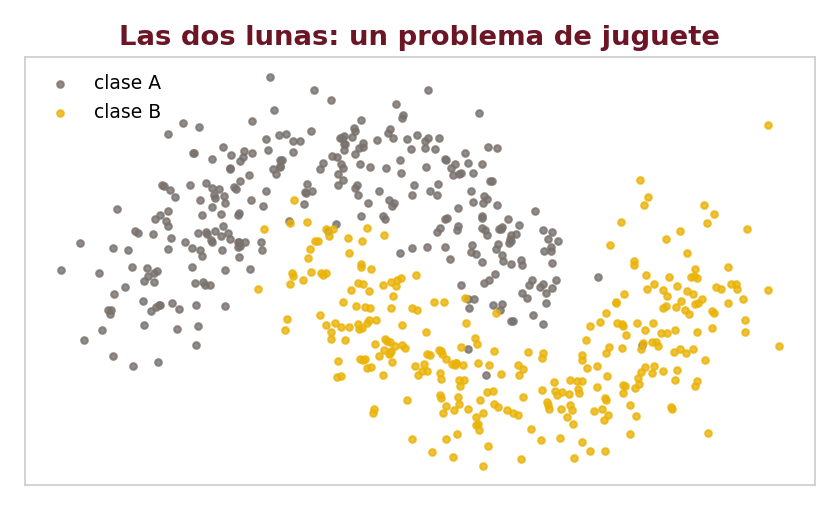
\includegraphics[width=0.94\textwidth]{fig_lunas.png}
    \end{column}
    \begin{column}{0.44\textwidth}
      {\footnotesize\color{textMuted}
      \begin{itemize}\setlength{\itemsep}{6pt}
        \item[{\color{arcaRed}\scriptsize\faArrowRight}]
          Dos grupos con forma de \textbf{medialunas
          entrelazadas}.
        \item[{\color{arcaRed}\scriptsize\faEye}]
          Cualquier persona los separa \textbf{a ojo},
          sin pensar.
        \item[{\color{arcaRed}\scriptsize\faQuestion}]
          Pregunta: ¿puede separarlos una \textbf{línea
          recta}?
      \end{itemize}
      }
      \vspace{4pt}
      {\scriptsize\color{arcaDark}\itshape
        Este dataset (\texttt{make\_moons}) es el examen
        clásico de no linealidad en ML.}
    \end{column}
  \end{columns}
\end{frame}

% ── LOGÍSTICA FRACASA ────────────────────────────────────────────────────────
\begin{frame}[shrink=5]{La Recta Fracasa; el Árbol lo Resuelve}
  \vspace{-6pt}
  {\small\color{arcaDark}\bfseries
    La regresión logística solo puede trazar una \textbf{frontera recta}. Miren lo que pasa.}

  \vspace{4pt}
  \centering
  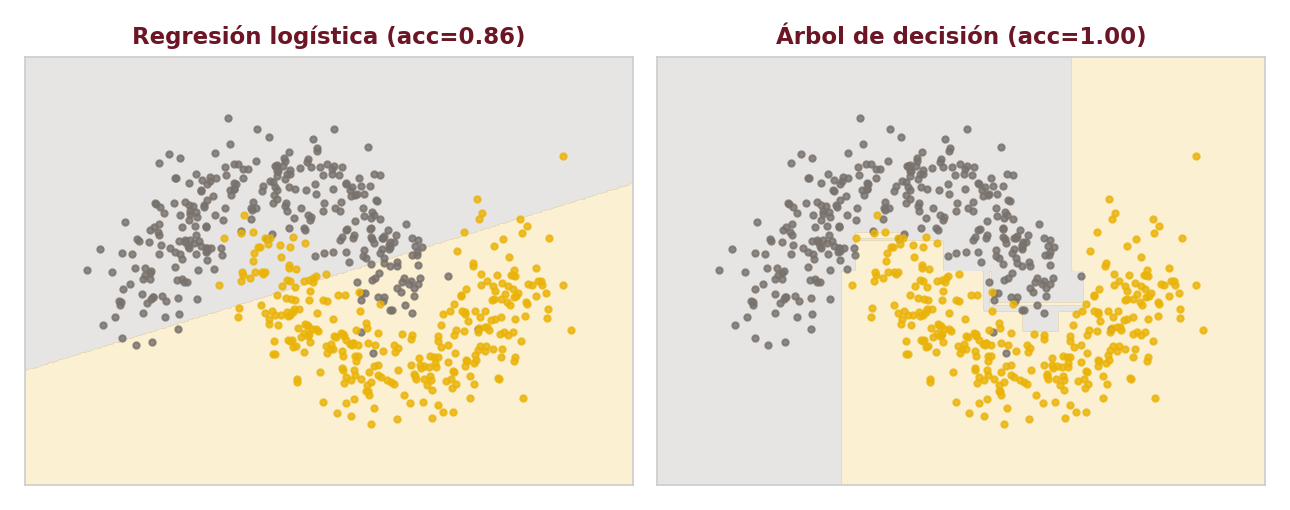
\includegraphics[width=0.86\textwidth,height=0.54\textheight,keepaspectratio]{fig_lunas_fronteras.png}

  \vspace{6pt}
  {\footnotesize\color{textMuted}
  \begin{itemize}\setlength{\itemsep}{3pt}
    \item[{\color{arcaRed}\scriptsize\faTimes}]
      La logística se queda en \textbf{0.86}: su recta corta las dos lunas
      por la mitad, \textbf{no puede hacer nada mejor}.
    \item[{\color{codeGreen}\scriptsize\faCheck}]
      El árbol dibuja una frontera de \textbf{escalones} que sigue la forma:
      \textbf{1.00}. Hoy aprenderemos cómo.
  \end{itemize}
  }
\end{frame}

\begin{frame}[shrink=5]{No es Solo una Luna: También Puede Haber Círculos}
  \vspace{-6pt}
  {\small\color{arcaDark}\bfseries
    Dos patrones fáciles para una persona, imposibles de separar perfectamente con una sola recta.}

  \vspace{2pt}
  \centering
  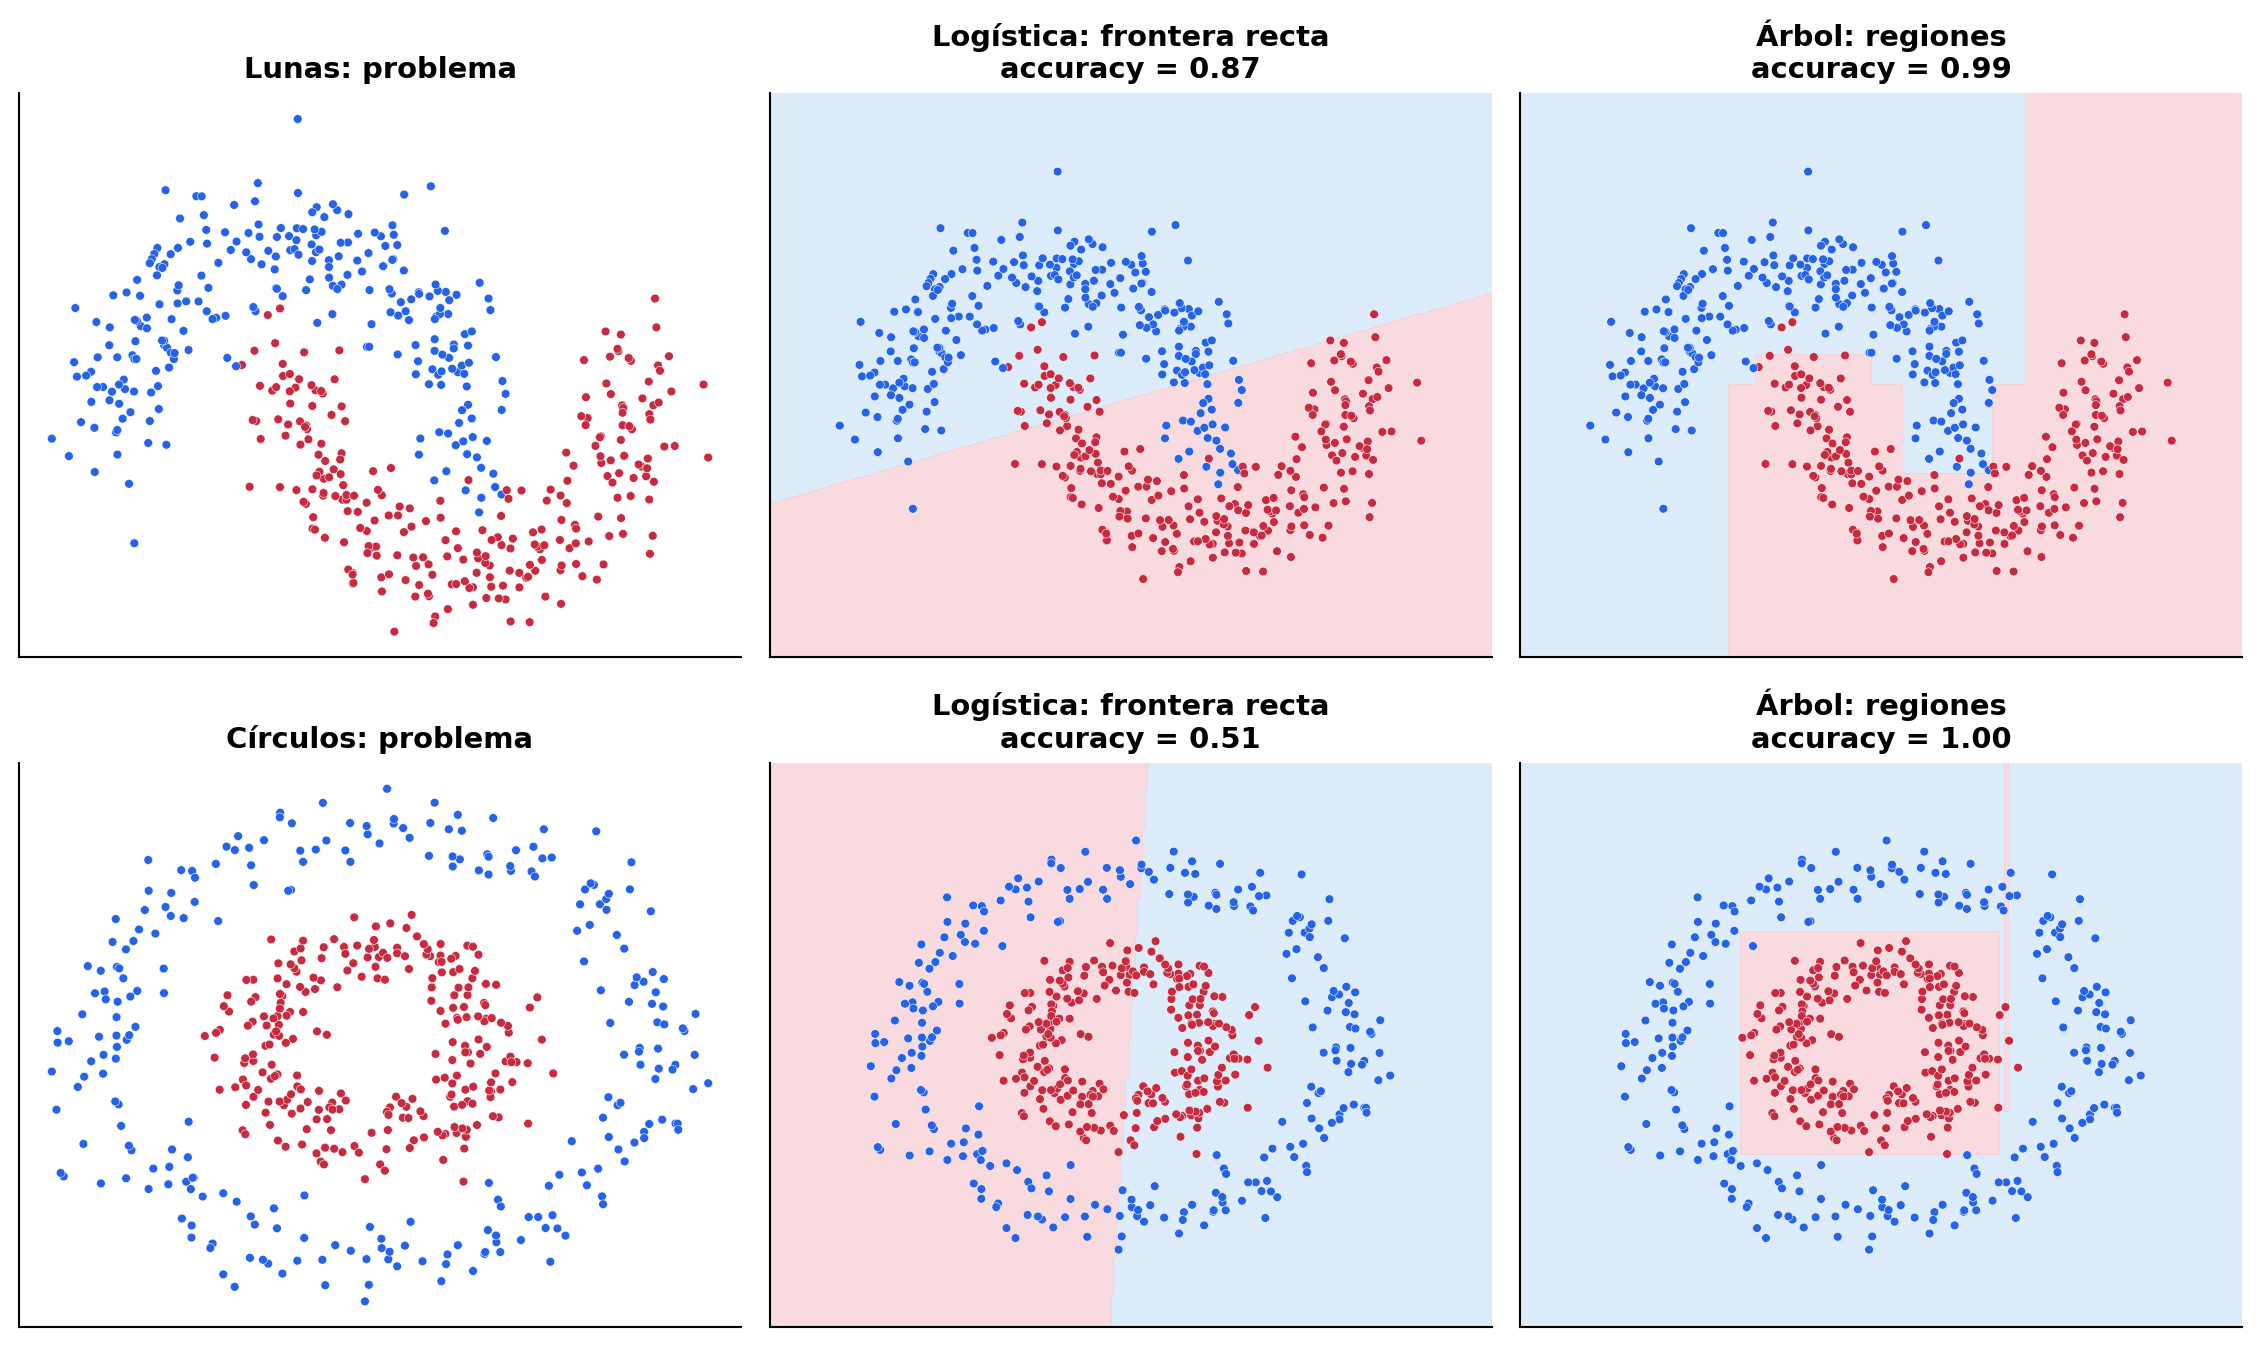
\includegraphics[width=0.88\textwidth,height=0.63\textheight,keepaspectratio]{fig_lunas_circulos.png}

  \vspace{2pt}
  {\scriptsize\color{textMuted}
    El árbol no dibuja una curva suave: combina muchos cortes horizontales y verticales
    hasta formar \textbf{regiones}. Esa es su manera de ``doblar''.}
\end{frame}

% ═════════════════════════════════════════════════════════════════════════════
\sectionframe{El Problema de Hoy}{Un medidor virtual de flujo}
% ═════════════════════════════════════════════════════════════════════════════

% ── EL PROBLEMA DE NEGOCIO ───────────────────────────────────────────────────
\begin{frame}[shrink=8]{¿Cuánto Está Produciendo Cada Pozo, Ahora?}
  \vspace{-4pt}
  {\small\color{arcaDark}\bfseries
    Parece una pregunta obvia. No lo es.}

  \vspace{6pt}
  \begin{columns}[T]
    \begin{column}{0.52\textwidth}
      {\footnotesize\color{textMuted}
      \begin{itemize}\setlength{\itemsep}{6pt}
        \item[{\color{arcaRed}\scriptsize\faFlask}]
          Medir el caudal de \textbf{un} pozo exige desviar su flujo
          al \textbf{separador de prueba}: se hace cada tantos
          días, \textbf{no} a diario.
        \item[{\color{arcaRed}\scriptsize\faClock}]
          Lo que \textbf{sí} está siempre disponible: los sensores
          de \textbf{presión}, \textbf{temperatura} y \textbf{choke}.
        \item[{\color{codeGreen}\scriptsize\faLightbulb}]
          \textbf{La idea:} un modelo que \textbf{estime la producción}
          desde esos sensores --- un \textit{medidor virtual de flujo}.
      \end{itemize}
      }
    \end{column}
    \begin{column}{0.44\textwidth}
      \begin{tcolorbox}[colback=arcaGray, colframe=arcaRed, boxrule=0pt, leftrule=3pt,
        arc=3pt, left=6pt, right=6pt, top=5pt, bottom=5pt]
        {\scriptsize\color{arcaDark}\bfseries Esto es un producto real:}\\[4pt]
        {\scriptsize\color{textMuted}
          los \textit{virtual flow meters} se venden y operan
          en la industria hoy. Detrás hay exactamente
          lo que vamos a construir: un modelo entrenado
          con datos históricos de pruebas de pozo.}
      \end{tcolorbox}
      \vspace{5pt}
      {\scriptsize\color{textMuted}\itshape
        Es \textbf{regresión} (predecimos un número), pero
        hoy la física no nos va a dejar usar una recta.}
    \end{column}
  \end{columns}
\end{frame}

% ── EL DATASET ───────────────────────────────────────────────────────────────
\begin{frame}[fragile,shrink=25]{El Dataset: Operación Diaria de Volve}
  \vspace{-4pt}
  {\small\color{arcaDark}\bfseries
    5 pozos productores de Volve, 7\,862 días de operación con sus sensores y su producción medida.}

  \vspace{4pt}
  \begin{columns}[T]
    \begin{column}{0.46\textwidth}
      \begin{pyblock}
op = pd.read_csv(url)
op.shape
      \end{pyblock}
      \vspace{2pt}
      \begin{outputblock}[]
(7862, 9)
      \end{outputblock}
    \end{column}
    \begin{column}{0.50\textwidth}
      {\scriptsize\color{textMuted}
      \begin{itemize}\setlength{\itemsep}{4pt}
        \item[{\color{arcaRed}\scriptsize\faDatabase}]
          El mismo campo Volve de las clases anteriores,
          ahora sus datos \textbf{de operación}.
        \item[{\color{codeGreen}\scriptsize\faCheck}]
          El target \texttt{oil} viene de las \textbf{mediciones
          reales} de producción diaria.
      \end{itemize}
      }
    \end{column}
  \end{columns}

  \vspace{4pt}
  \centering
  {\scriptsize
  \renewcommand{\arraystretch}{1.3}
  \begin{tabular}{@{}l l l@{}}
    \toprule
    {\bfseries\color{arcaRed} Columna} & {\bfseries\color{arcaDark} Qué mide} & {\bfseries\color{arcaDark} Dónde se mide} \\
    \midrule
    \texttt{p\_fondo} & presión en el fondo del pozo (bar) & sensor de fondo \\
    \texttt{p\_cabeza} & presión en la cabeza del pozo (bar) & superficie \\
    \texttt{t\_cabeza} & temperatura en cabeza (\(^{\circ}\)C) & superficie \\
    \texttt{choke} & apertura de la válvula choke (\%) & superficie \\
    \texttt{dp\_choke} & caída de presión a través del choke & superficie \\
    \texttt{horas} & horas en operación ese día & registro \\
    \midrule
    \texttt{oil} & \textbf{el target}: producción (Sm\(^3\)/día) & separador \\
    \bottomrule
  \end{tabular}
  }
\end{frame}

% ── EXPLORAR: LA CURVA ───────────────────────────────────────────────────────
\begin{frame}{Explorar: la Relación Más Fuerte\ldots es Curva}
  \vspace{-6pt}
  {\small\color{arcaDark}\bfseries
    La correlación más alta con \texttt{oil} es \texttt{p\_cabeza} (0.64). Dibujémosla.}

  \vspace{4pt}
  \begin{columns}[T]
    \begin{column}{0.54\textwidth}
      \centering
      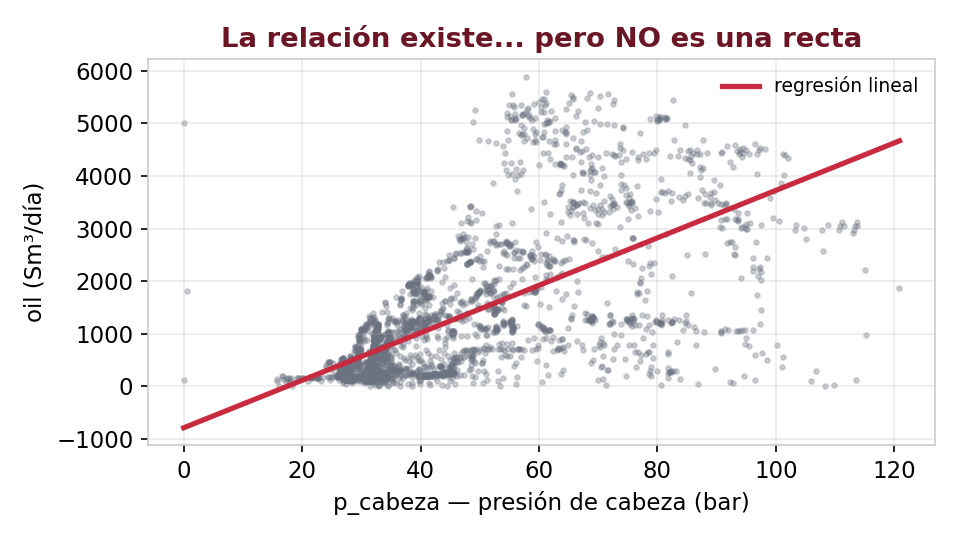
\includegraphics[width=\textwidth]{fig_curva_real.png}
    \end{column}
    \begin{column}{0.42\textwidth}
      {\footnotesize\color{textMuted}
      \begin{itemize}\setlength{\itemsep}{6pt}
        \item[{\color{arcaRed}\scriptsize\faArrowRight}]
          Hay relación, clarísima. Pero la nube tiene
          \textbf{forma de codo}, no de recta.
        \item[{\color{arcaRed}\scriptsize\faTimes}]
          La recta pasa \textbf{por en medio de nada}:
          subestima abajo, sobreestima arriba.
        \item[{\color{arcaRed}\scriptsize\faExclamationTriangle}]
          Y esto es \textbf{una sola} variable: las interacciones
          entre presiones y choke lo complican más.
      \end{itemize}
      }
    \end{column}
  \end{columns}
\end{frame}

% ── LA LINEAL SE QUEDA CORTA ─────────────────────────────────────────────────
\begin{frame}[fragile,shrink=20]{La Regresión Lineal se Queda Corta}
  \vspace{-4pt}
  {\small\color{arcaDark}\bfseries
    Entrenamos la lineal de la Clase 1 con las 6 variables. El resultado:}

  \vspace{4pt}
  \begin{columns}[T]
    \begin{column}{0.52\textwidth}
      \begin{pyblock}
lineal = LinearRegression()
lineal.fit(X_tr, y_tr)

r2 = lineal.score(X_te, y_te)
print("R2:", r2)
      \end{pyblock}
      \vspace{2pt}
      \begin{outputblock}
R2: 0.595
MAE: 583 Sm3/dia
      \end{outputblock}
    \end{column}
    \begin{column}{0.44\textwidth}
      {\scriptsize\color{textMuted}
      \begin{itemize}\setlength{\itemsep}{5pt}
        \item[{\color{arcaRed}\scriptsize\faTimes}]
          Explica el \textbf{60\,\%} y se equivoca
          \textbf{583 Sm\(^3\)/día} en promedio ---
          casi \textbf{la mitad} de la producción
          media (1\,264).
        \item[{\color{arcaRed}\scriptsize\faArrowRight}]
          No es que el problema sea impredecible:
          es que \textbf{la recta no puede doblar}.
        \item[{\color{codeGreen}\scriptsize\faLightbulb}]
          Necesitamos un modelo que capture
          \textbf{curvas y umbrales}.
      \end{itemize}
      }
    \end{column}
  \end{columns}
\end{frame}

% ═════════════════════════════════════════════════════════════════════════════
\sectionframe{Árboles de Decisión}{Cutoffs automatizados}
% ═════════════════════════════════════════════════════════════════════════════

% ── USTEDES YA PIENSAN EN ÁRBOLES ────────────────────────────────────────────
\begin{frame}{Ustedes Ya Piensan en Árboles}
  \vspace{-6pt}
  {\small\color{arcaDark}\bfseries
    Un cutoff es una decisión con umbral. Los usan todos los días.}

  \vspace{8pt}
  \begin{columns}[T]
    \begin{column}{0.48\textwidth}
      {\footnotesize\color{textMuted}
      \begin{itemize}\setlength{\itemsep}{7pt}
        \item[{\color{arcaRed}\scriptsize\faCodeBranch}]
          ``Si el \texttt{GR} \(<\) 60 \(\to\) arena; si no \(\to\) arcilla.''
        \item[{\color{arcaRed}\scriptsize\faCodeBranch}]
          ``Si la presión anular \(>\) X \(\to\) revisar; si no \(\to\) seguir.''
        \item[{\color{arcaRed}\scriptsize\faCodeBranch}]
          Y los encadenan: ``si es arena \textbf{y} la porosidad
          \(>\) 15\,\% \textbf{y} la resistividad es alta \(\to\) zona de interés.''
      \end{itemize}
      }
    \end{column}
    \begin{column}{0.48\textwidth}
      \begin{tcolorbox}[colback=arcaGray, colframe=arcaRed, boxrule=0pt, leftrule=3pt,
        arc=3pt, left=6pt, right=6pt, top=5pt, bottom=5pt]
        {\scriptsize\color{arcaDark}\bfseries Un árbol de decisión es exactamente eso:}\\[4pt]
        {\scriptsize\color{textMuted}
          una \textbf{cascada de cutoffs}\ldots{} con una diferencia:
          \textbf{la máquina elige los cortes} --- qué variable,
          en qué valor y en qué orden --- probando miles de
          opciones y quedándose con las que \textbf{mejor separan}
          los datos.}
      \end{tcolorbox}
      \vspace{5pt}
      {\scriptsize\color{textMuted}\itshape
        No hay fórmula ni coeficientes: solo preguntas
        de sí/no encadenadas.}
    \end{column}
  \end{columns}
\end{frame}

% ── ANATOMÍA, ANTES DEL ÁRBOL REAL ───────────────────────────────────────────
\begin{frame}{Anatomía de un Árbol: Cuatro Palabras}
  \vspace{-5pt}
  \begin{columns}[T]
    \begin{column}{0.57\textwidth}
      \centering
      \begin{tikzpicture}[
        level distance=1.45cm,
        level 1/.style={sibling distance=4.1cm},
        level 2/.style={sibling distance=2.0cm},
        every node/.style={font=\scriptsize,align=center},
        q/.style={draw=arcaRed,rounded corners,fill=arcaRed!10,
          minimum width=2.7cm,minimum height=.72cm},
        leaf/.style={draw=codeGreen,rounded corners,fill=codeGreen!10,
          minimum width=1.65cm,minimum height=.65cm}]
        \node[q] (root) {¿presión $\leq 46$?}
          child {node[q] {¿choke $\leq 55$?}
            child {node[leaf] {603\\Sm$^3$/día}}
            child {node[leaf] {1\,020\\Sm$^3$/día}}}
          child {node[leaf] {2\,461\\Sm$^3$/día}};
        \node[anchor=east,text=arcaRed,font=\scriptsize\bfseries] at ([xshift=-.25cm]root.west) {nodo};
        \node[text=textMuted,font=\tiny] at (-1.15,-.75) {rama: sí};
        \node[text=textMuted,font=\tiny] at (1.15,-.75) {rama: no};
        \node[text=codeGreen,font=\scriptsize\bfseries] at (3.2,-2.8) {hoja};
      \end{tikzpicture}
    \end{column}
    \begin{column}{0.39\textwidth}
      {\footnotesize\color{textMuted}
      \begin{itemize}\setlength{\itemsep}{7pt}
        \item \textbf{\color{arcaRed}Raíz:} la primera pregunta.
        \item \textbf{\color{arcaRed}Nodo:} una pregunta intermedia.
        \item \textbf{\color{arcaRed}Rama:} la respuesta sí/no.
        \item \textbf{\color{codeGreen}Hoja:} la predicción final.
      \end{itemize}}
      \vspace{5pt}
      {\scriptsize\color{arcaDark}\itshape
        Leer un árbol es seguir una ruta, no resolver una ecuación.}
    \end{column}
  \end{columns}
\end{frame}

\begin{frame}{¿Cómo Decide la Primera Pregunta?}
  \vspace{-6pt}
  {\small\color{arcaDark}\bfseries
    Prueba muchos candidatos y conserva el corte que deja grupos más homogéneos.}

  \vspace{3pt}
  \centering
  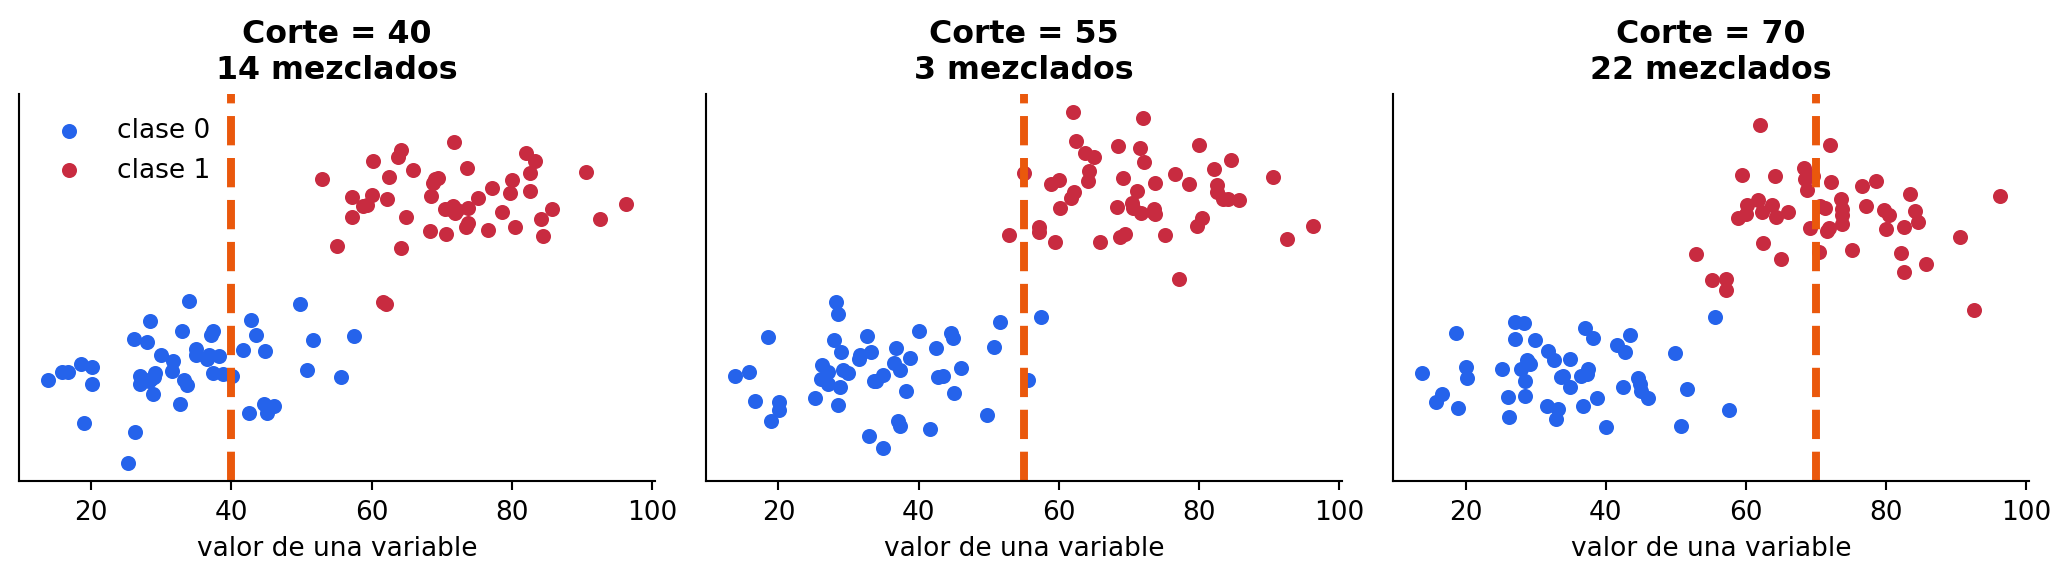
\includegraphics[width=0.89\textwidth]{fig_candidatos_corte.png}

  \vspace{4pt}
  {\footnotesize\color{textMuted}
    Para cada variable prueba distintos valores. En clasificación busca grupos con
    \textbf{menos mezcla}; en regresión, grupos con valores \textbf{menos dispersos}.}
\end{frame}

\begin{frame}{La Misma Mecánica, Dos Tipos de Predicción}
  \vspace{-5pt}
  \begin{columns}[T]
    \begin{column}{0.47\textwidth}
      \begin{tcolorbox}[colback=arcaGray,colframe=codeBlue,boxrule=0pt,
        leftrule=3pt,arc=3pt,left=7pt,right=7pt,top=7pt,bottom=7pt]
        {\small\color{codeBlue}\bfseries Árbol de regresión}\\[6pt]
        {\footnotesize\color{textMuted}
          Llegan a una hoja estos caudales:\\
          580, 620, 610, 590\\[5pt]
          Predicción = \textbf{promedio}\\
          Predicción final: \textbf{600 Sm\(^3\)/día}.}
      \end{tcolorbox}
    \end{column}
    \begin{column}{0.47\textwidth}
      \begin{tcolorbox}[colback=arcaGray,colframe=arcaRed,boxrule=0pt,
        leftrule=3pt,arc=3pt,left=7pt,right=7pt,top=7pt,bottom=7pt]
        {\small\color{arcaRed}\bfseries Árbol de clasificación}\\[6pt]
        {\footnotesize\color{textMuted}
          Llegan a una hoja 8 arenas y 2 lutitas.\\[5pt]
          Clase = \textbf{voto mayoritario}: arena\\
          Probabilidad = \textbf{8/10 = 0.80}}
      \end{tcolorbox}
    \end{column}
  \end{columns}
  \vspace{9pt}
  \centering
  {\small\color{arcaDark}\bfseries
    Cambia lo que ocurre en la hoja; la secuencia de preguntas es la misma.}
\end{frame}

\begin{frame}{¿Cuándo Deja de Preguntar?}
  \vspace{-6pt}
  {\small\color{arcaDark}\bfseries
    Si no ponemos límites, el árbol puede crear una hoja para casi cada ejemplo.}

  \vspace{6pt}
  \begin{columns}[T]
    \begin{column}{0.31\textwidth}
      \begin{tcolorbox}[colback=arcaGray,colframe=arcaRed,boxrule=0pt,leftrule=3pt,arc=3pt]
        {\scriptsize\bfseries\color{arcaRed}max\_depth}\\[4pt]
        {\scriptsize\color{textMuted}Máximo número de niveles. Controla cuánto puede complicarse.}
      \end{tcolorbox}
    \end{column}
    \begin{column}{0.31\textwidth}
      \begin{tcolorbox}[colback=arcaGray,colframe=codeBlue,boxrule=0pt,leftrule=3pt,arc=3pt]
        {\scriptsize\bfseries\color{codeBlue}min\_samples\_leaf}\\[4pt]
        {\scriptsize\color{textMuted}Mínimo de ejemplos que debe contener una hoja.}
      \end{tcolorbox}
    \end{column}
    \begin{column}{0.31\textwidth}
      \begin{tcolorbox}[colback=arcaGray,colframe=codeGreen,boxrule=0pt,leftrule=3pt,arc=3pt]
        {\scriptsize\bfseries\color{codeGreen}min\_samples\_split}\\[4pt]
        {\scriptsize\color{textMuted}Mínimo de ejemplos para permitir una nueva pregunta.}
      \end{tcolorbox}
    \end{column}
  \end{columns}
  \vspace{10pt}
  {\footnotesize\color{textMuted}
    No buscamos el árbol que mejor recuerde el entrenamiento. Buscamos el más simple
    que conserve buen desempeño en \textbf{datos nuevos}.}
\end{frame}

% ── EL ÁRBOL REAL ────────────────────────────────────────────────────────────
\begin{frame}{Nuestro Primer Árbol, Dibujado}
  \vspace{-6pt}
  {\small\color{arcaDark}\bfseries
    Un árbol de \textbf{2 niveles} entrenado con nuestros datos. Se lee de arriba hacia abajo.}

  \vspace{2pt}
  \centering
  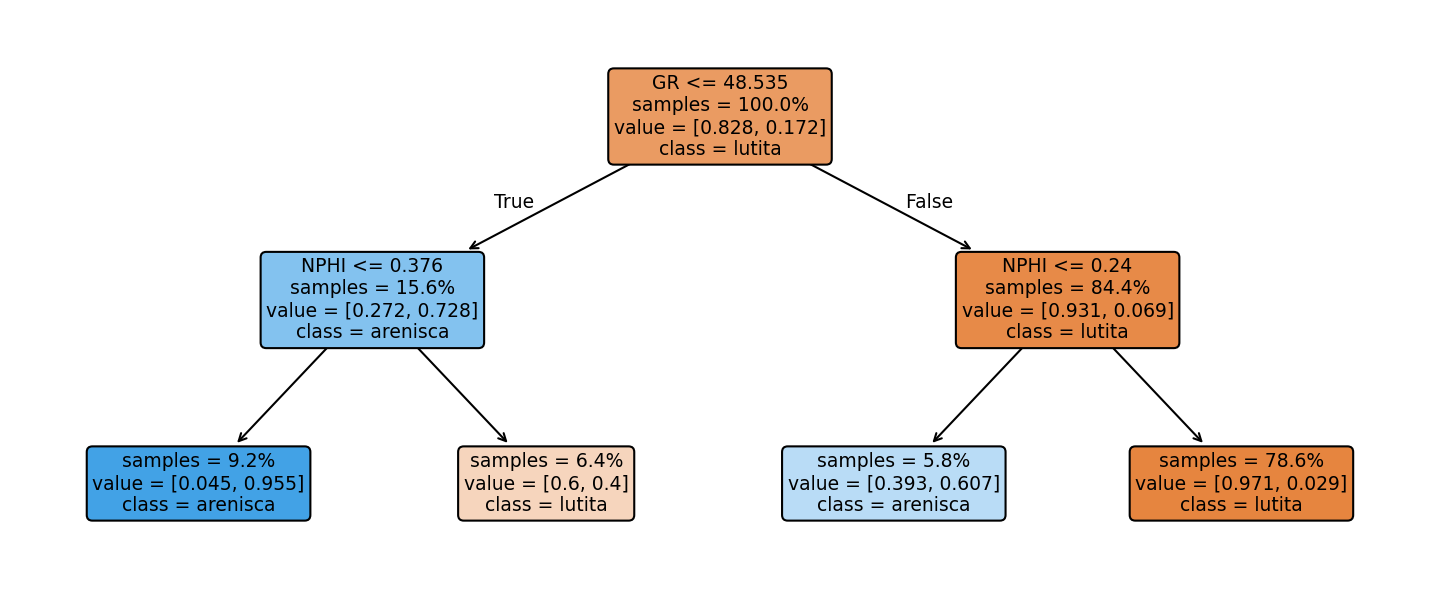
\includegraphics[width=0.80\textwidth,height=0.54\textheight,keepaspectratio]{fig_arbol_diagrama.png}

  \vspace{4pt}
  {\footnotesize\color{textMuted}
  \begin{itemize}\setlength{\itemsep}{2pt}
    \item[{\color{arcaRed}\scriptsize\faArrowRight}]
      Primera pregunta: ¿\texttt{p\_cabeza} \(\leq\) 46? Si sí, el pozo produce
      poco (\(\sim\)603); si no, mucho (\(\sim\)2\,461).
    \item[{\color{codeGreen}\scriptsize\faCheck}]
      Con solo \textbf{3 preguntas}, este árbol ya da R\textsuperscript{2} = 0.66:
      \textbf{le gana a la regresión lineal con sus 6 variables}.
  \end{itemize}
  }
\end{frame}

% ── CÓMO SE ADAPTA ───────────────────────────────────────────────────────────
\begin{frame}{Por Qué el Árbol Captura lo No Lineal}
  \vspace{-6pt}
  {\small\color{arcaDark}\bfseries
    Cada corte crea un ``escalón''. Muchos escalones siguen cualquier curva.}

  \vspace{4pt}
  \begin{columns}[T]
    \begin{column}{0.54\textwidth}
      \centering
      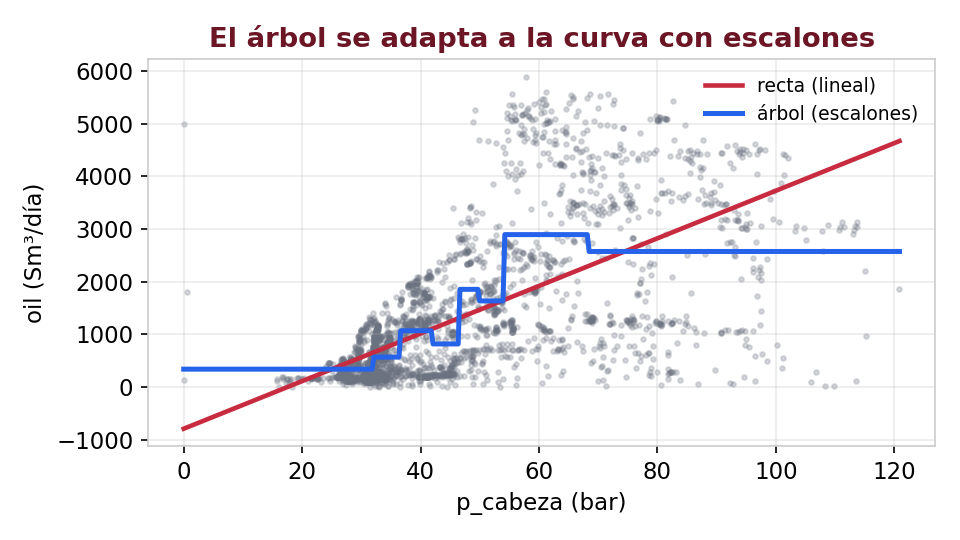
\includegraphics[width=\textwidth]{fig_arbol_1d.png}
    \end{column}
    \begin{column}{0.42\textwidth}
      {\footnotesize\color{textMuted}
      \begin{itemize}\setlength{\itemsep}{6pt}
        \item[{\color{arcaRed}\scriptsize\faArrowRight}]
          La \textbf{recta} está obligada a mantener la misma
          pendiente en todas partes.
        \item[{\color{codeBlue}\scriptsize\faArrowRight}]
          El \textbf{árbol} predice un valor distinto en cada
          tramo: donde la curva sube rápido, pone
          escalones altos.
        \item[{\color{codeGreen}\scriptsize\faCheck}]
          Sin decirle nada de la física: los cortes salen
          \textbf{de los datos}.
      \end{itemize}
      }
    \end{column}
  \end{columns}
\end{frame}

% ── EN CÓDIGO ────────────────────────────────────────────────────────────────
\begin{frame}[fragile,shrink=22]{En Código: el Mismo Patrón de Siempre}
  \vspace{-4pt}
  {\small\color{arcaDark}\bfseries
    Cambia el modelo, no el flujo. Y un detalle cómodo: los árboles \textbf{no necesitan estandarización}.}

  \vspace{4pt}
  \begin{columns}[T]
    \begin{column}{0.54\textwidth}
      \begin{pyblock}
from sklearn.tree import DecisionTreeRegressor

arbol = DecisionTreeRegressor(
    max_depth=5, random_state=42)
arbol.fit(X_tr, y_tr)

print(arbol.score(X_te, y_te))
      \end{pyblock}
      \vspace{2pt}
      \begin{outputblock}
0.886
      \end{outputblock}
    \end{column}
    \begin{column}{0.42\textwidth}
      {\scriptsize\color{textMuted}
      \begin{itemize}\setlength{\itemsep}{5pt}
        \item[{\color{codeGreen}\scriptsize\faCheck}]
          De 0.60 a \textbf{0.89} con 5 niveles de preguntas.
        \item[{\color{arcaRed}\scriptsize\faArrowRight}]
          \texttt{max\_depth}: cuántos niveles de preguntas
          puede hacer. Es \textbf{la perilla clave}.
        \item[{\color{arcaRed}\scriptsize\faArrowRight}]
          Los cortes comparan cada variable \textbf{consigo
          misma} \(\to\) las escalas no importan.
      \end{itemize}
      }
    \end{column}
  \end{columns}
\end{frame}

% ── OVERFITTING ──────────────────────────────────────────────────────────────
\begin{frame}{La Tentación: ¿y si lo Dejamos Crecer Sin Límite?}
  \vspace{-6pt}
  {\small\color{arcaDark}\bfseries
    Más profundidad = más poder. Hasta que empieza a \textbf{memorizar}.}

  \vspace{4pt}
  \begin{columns}[T]
    \begin{column}{0.56\textwidth}
      \centering
      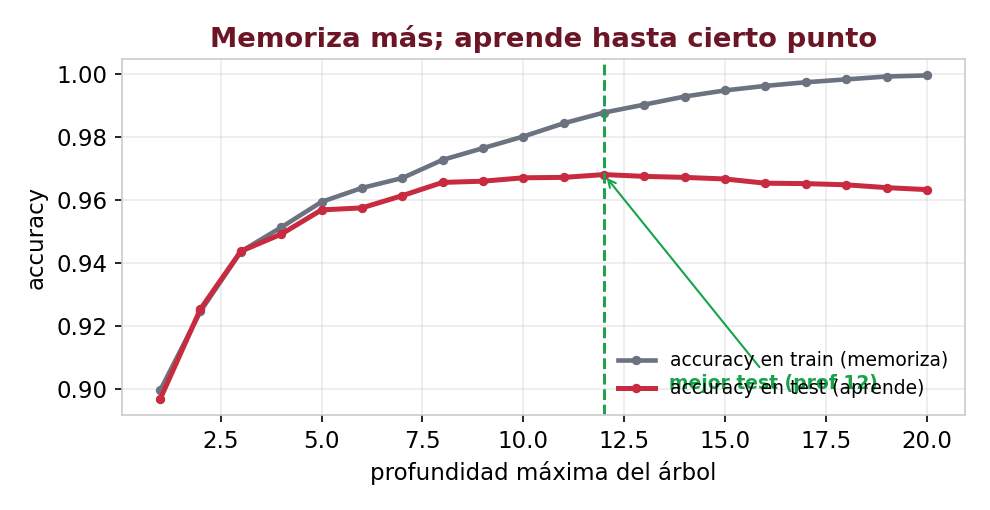
\includegraphics[width=\textwidth]{fig_overfit.png}
    \end{column}
    \begin{column}{0.40\textwidth}
      {\footnotesize\color{textMuted}
      \begin{itemize}\setlength{\itemsep}{5pt}
        \item[{\color{arcaRed}\scriptsize\faArrowRight}]
          Sin límite, el árbol memoriza \textbf{cada día}
          del historial: R\textsuperscript{2} \textbf{train} = 1.000.
        \item[{\color{arcaRed}\scriptsize\faExclamationTriangle}]
          Pero en \textbf{test} no mejora más: aprendió
          el \textbf{ruido}, no el patrón.
        \item[{\color{codeGreen}\scriptsize\faCheck}]
          Es el \textbf{overfitting} de la Clase 1, ahora
          \textbf{visible} en una curva.
      \end{itemize}
      }
    \end{column}
  \end{columns}

  \vspace{2pt}
  {\scriptsize\color{textMuted}
    \faLightbulb[regular]\hspace{3pt}%
    El árbol solo es \textbf{poderoso pero indisciplinado}. La solución no es un árbol mejor\ldots{}
    son \textbf{muchos árboles}.}
\end{frame}

% ═════════════════════════════════════════════════════════════════════════════
\sectionframe{Random Forest}{La sabiduría de la multitud}
% ═════════════════════════════════════════════════════════════════════════════

% ── LA IDEA ──────────────────────────────────────────────────────────────────
\begin{frame}{La Idea: Preguntarle a 200 Ingenieros Distintos}
  \vspace{-6pt}
  {\small\color{arcaDark}\bfseries
    Un experto se equivoca. El \textbf{promedio de muchos expertos independientes} se equivoca mucho menos.}

  \vspace{8pt}
  \begin{columns}[T]
    \begin{column}{0.50\textwidth}
      {\footnotesize\color{textMuted}
      \begin{itemize}\setlength{\itemsep}{7pt}
        \item[{\color{arcaRed}\scriptsize\faTree}]
          \textbf{Random Forest} entrena \textbf{cientos de árboles},
          cada uno un poco distinto.
        \item[{\color{arcaRed}\scriptsize\faRandom}]
          ¿Distintos cómo? Cada árbol ve una \textbf{muestra
          distinta de los días} y considera \textbf{variables
          distintas} en cada corte.
        \item[{\color{arcaRed}\scriptsize\faUsers}]
          La predicción final: el \textbf{promedio} de todos
          (o el voto, si es clasificación).
      \end{itemize}
      }
    \end{column}
    \begin{column}{0.46\textwidth}
      \begin{tcolorbox}[colback=arcaGray, colframe=codeGreen, boxrule=0pt, leftrule=3pt,
        arc=3pt, left=6pt, right=6pt, top=5pt, bottom=5pt]
        {\scriptsize\color{arcaDark}\bfseries Por qué funciona:}\\[4pt]
        {\scriptsize\color{textMuted}
          cada árbol memoriza \textbf{ruido distinto}. Al
          promediar, los errores individuales
          \textbf{se cancelan entre sí} y queda el patrón
          que todos vieron: \textbf{la señal}.}
      \end{tcolorbox}
      \vspace{5pt}
      {\scriptsize\color{textMuted}\itshape
        Como promediar las estimaciones de 200
        ingenieros que estudiaron el campo
        con informes diferentes.}
    \end{column}
  \end{columns}
\end{frame}

% ── RF EN CÓDIGO ─────────────────────────────────────────────────────────────
\begin{frame}[fragile,shrink=22]{Random Forest en Código}
  \vspace{-4pt}
  {\small\color{arcaDark}\bfseries
    Una línea distinta. El resto del flujo, idéntico.}

  \vspace{4pt}
  \begin{columns}[T]
    \begin{column}{0.54\textwidth}
      \begin{pyblock}
from sklearn.ensemble import RandomForestRegressor

bosque = RandomForestRegressor(
    n_estimators=200, random_state=42)
bosque.fit(X_tr, y_tr)

print(bosque.score(X_te, y_te))
      \end{pyblock}
      \vspace{2pt}
      \begin{outputblock}
0.980
      \end{outputblock}
    \end{column}
    \begin{column}{0.42\textwidth}
      {\scriptsize\color{textMuted}
      \begin{itemize}\setlength{\itemsep}{5pt}
        \item[{\color{arcaRed}\scriptsize\faArrowRight}]
          \texttt{n\_estimators}: cuántos árboles.
          200 es un buen punto de partida.
        \item[{\color{codeGreen}\scriptsize\faCheck}]
          \textbf{R\textsuperscript{2} = 0.98} en datos que nunca vio.
        \item[{\color{codeGreen}\scriptsize\faCheck}]
          Y sin estandarizar, sin transformar,
          sin decirle nada de la física.
      \end{itemize}
      }
    \end{column}
  \end{columns}
\end{frame}

% ── LA COMPARACIÓN ───────────────────────────────────────────────────────────
\begin{frame}{El Marcador Final}
  \vspace{-6pt}
  {\small\color{arcaDark}\bfseries
    Mismo problema, mismos datos de test. Solo cambió el modelo.}

  \vspace{4pt}
  \begin{columns}[T]
    \begin{column}{0.54\textwidth}
      \centering
      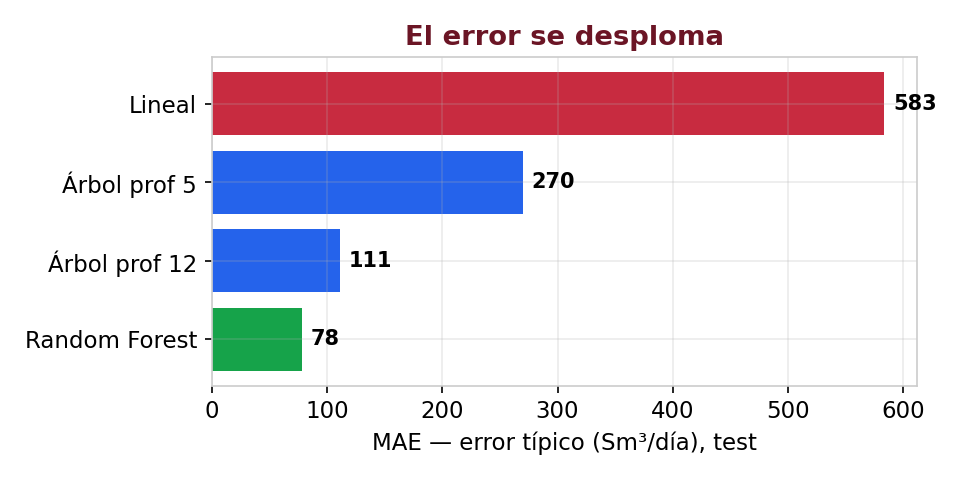
\includegraphics[width=\textwidth]{fig_comparacion.png}
    \end{column}
    \begin{column}{0.42\textwidth}
      {\footnotesize
      \renewcommand{\arraystretch}{1.4}
      \begin{tabular}{@{}l c c@{}}
        \toprule
        & {\bfseries\color{arcaDark} R\textsuperscript{2}} & {\bfseries\color{arcaDark} MAE} \\
        \midrule
        Lineal & 0.60 & 583 \\
        Árbol p5 & 0.89 & 270 \\
        Árbol p12 & 0.96 & 111 \\
        \rowcolor{arcaGray}
        \textbf{R.\ Forest} & \textbf{0.98} & \textbf{78} \\
        \bottomrule
      \end{tabular}
      }
      \vspace{6pt}
      {\scriptsize\color{textMuted}
        El error típico bajó de \textbf{583} a \textbf{78}
        Sm\(^3\)/día: \textbf{7.5 veces menos}.\\[4pt]
        \itshape Para un pozo de 1\,264 Sm\(^3\)/día de media,
        es pasar de inutilizable a operativo.}
    \end{column}
  \end{columns}
\end{frame}

% ── PREDICHO VS REAL ─────────────────────────────────────────────────────────
\begin{frame}{El Veredicto Visual}
  \vspace{-6pt}
  {\small\color{arcaDark}\bfseries
    Predicho vs real en el test: el medidor virtual funciona.}

  \vspace{2pt}
  \begin{columns}[T]
    \begin{column}{0.50\textwidth}
      \centering
      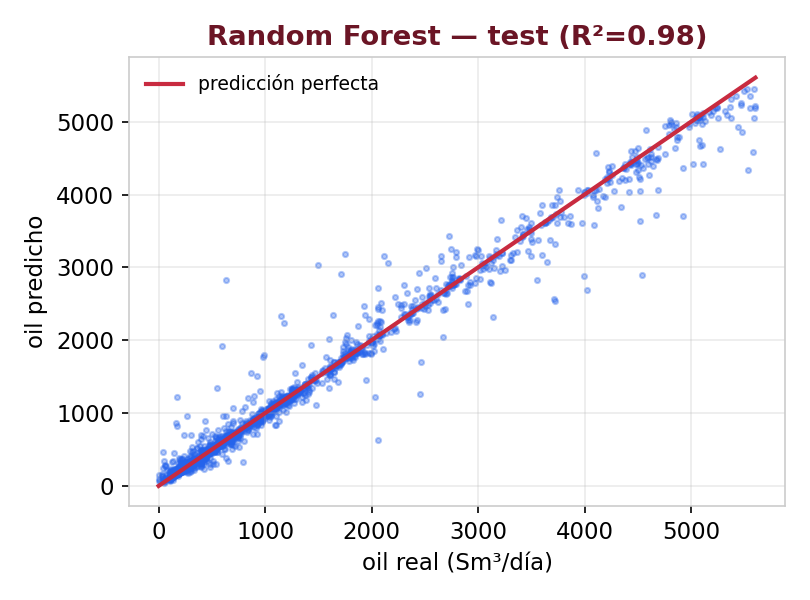
\includegraphics[width=0.9\textwidth]{fig_pred_real_rf.png}
    \end{column}
    \begin{column}{0.46\textwidth}
      {\footnotesize\color{textMuted}
      \begin{itemize}\setlength{\itemsep}{6pt}
        \item[{\color{codeGreen}\scriptsize\faCheck}]
          Los puntos se pegan a la diagonal en \textbf{todo}
          el rango: días de 200 y días de 5\,000 Sm\(^3\).
        \item[{\color{arcaRed}\scriptsize\faArrowRight}]
          Recuerden la Clase 1: la recta del declive
          predecía \textbf{producción negativa}. El bosque
          no comete esos absurdos: nunca predice fuera
          del rango que vio.
      \end{itemize}
      }
    \end{column}
  \end{columns}
\end{frame}

% ── IMPORTANCIA ──────────────────────────────────────────────────────────────
\begin{frame}{¿En Qué se Fija el Bosque?}
  \vspace{-6pt}
  {\small\color{arcaDark}\bfseries
    El bosque no da coeficientes, pero sí dice \textbf{cuánto usó} cada variable.}

  \vspace{4pt}
  \begin{columns}[T]
    \begin{column}{0.52\textwidth}
      \centering
      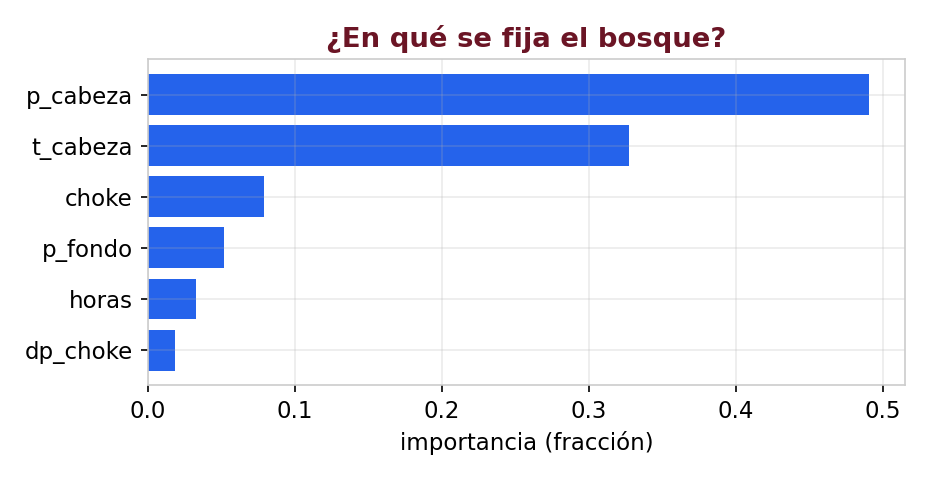
\includegraphics[width=\textwidth]{fig_importancia.png}
    \end{column}
    \begin{column}{0.44\textwidth}
      {\footnotesize\color{textMuted}
      \begin{itemize}\setlength{\itemsep}{6pt}
        \item[{\color{codeGreen}\scriptsize\faTrophy}]
          \texttt{p\_cabeza} (49\,\%) y \texttt{t\_cabeza} (33\,\%)
          dominan: la presión y temperatura de cabeza
          \textbf{son} la firma del caudal.
        \item[{\color{arcaRed}\scriptsize\faArrowRight}]
          Coincide con la física: lo que pasa por el choke
          se refleja en las condiciones de cabeza.
        \item[{\color{arcaRed}\scriptsize\faExclamationTriangle}]
          Ojo: importancia \(\neq\) causalidad. Dice qué
          \textbf{usó} el modelo, no qué \textbf{causa} el flujo.
      \end{itemize}
      }
    \end{column}
  \end{columns}
\end{frame}

% ── EL PRECIO ────────────────────────────────────────────────────────────────
\begin{frame}[shrink=8]{El Precio: Poder vs Explicabilidad}
  \vspace{-4pt}
  {\small\color{arcaDark}\bfseries
    Nada es gratis. Lo que ganamos en precisión lo pagamos en transparencia.}

  \vspace{6pt}
  \centering
  {\footnotesize
  \renewcommand{\arraystretch}{1.5}
  \begin{tabular}{@{}p{3.4cm} c c c@{}}
    \toprule
    & {\bfseries\color{arcaDark} Lineal/Logística} & {\bfseries\color{arcaDark} Árbol} & {\bfseries\color{arcaDark} R.\ Forest} \\
    \midrule
    \rowcolor{arcaGray}
    Captura curvas & \color{arcaRed}no & \color{codeGreen}sí & \color{codeGreen}sí \\
    Resiste overfitting & \color{codeGreen}sí & \color{arcaRed}no & \color{codeGreen}sí \\
    \rowcolor{arcaGray}
    Se explica completo & \color{codeGreen}sí (fórmula) & \color{codeGreen}sí (diagrama) & \color{arcaRed}no (200 árboles) \\
    Necesita estandarizar & sí & no & no \\
    \bottomrule
  \end{tabular}
  }

  \vspace{8pt}
  {\footnotesize\color{textMuted}
  \begin{itemize}\setlength{\itemsep}{4pt}
    \item[{\color{arcaRed}\scriptsize\faArrowRight}]
      Del bosque solo podemos explicar las \textbf{importancias}, no el camino de cada predicción.
    \item[{\color{codeGreen}\scriptsize\faCheck}]
      Por eso la práctica profesional: \textbf{empezar simple} (línea base explicable) y
      \textbf{escalar} solo si el negocio necesita la precisión extra.
  \end{itemize}
  }
\end{frame}

% ═════════════════════════════════════════════════════════════════════════════
\sectionframe{Segundo Problema: Clasificación}{Volvemos a FORCE 2020 con una frontera no lineal}
% ═════════════════════════════════════════════════════════════════════════════

\begin{frame}{La Pregunta es la Misma; el Modelo Ahora Puede Doblar}
  \vspace{-6pt}
  {\small\color{arcaDark}\bfseries
    Clase 2: con registros de pozo, decidir si una profundidad es arenisca o lutita.}

  \vspace{6pt}
  \begin{columns}[T]
    \begin{column}{0.49\textwidth}
      {\footnotesize\color{textMuted}
      \begin{itemize}\setlength{\itemsep}{7pt}
        \item \textbf{Dataset 2:} FORCE 2020, 62\,792 muestras de 11 pozos.
        \item \textbf{Features:} GR, RHOB, NPHI, DTC y RDEP.
        \item \textbf{Target:} arenisca = 1; lutita = 0.
        \item \textbf{Costo:} perder una arena cuesta 10 veces más que una falsa alarma.
      \end{itemize}}
    \end{column}
    \begin{column}{0.47\textwidth}
      \begin{tcolorbox}[colback=arcaGray,colframe=arcaRed,boxrule=0pt,
        leftrule=3pt,arc=3pt,left=7pt,right=7pt,top=7pt,bottom=7pt]
        {\small\color{arcaDark}\bfseries Lo nuevo}\\[5pt]
        {\footnotesize\color{textMuted}
          La logística busca una frontera plana.
          El árbol puede combinar reglas como:\\[5pt]
          \texttt{GR < corte}\\
          \textbf{y} \texttt{NPHI < corte}\\
          \textbf{y} \texttt{DTC < corte}}
      \end{tcolorbox}
    \end{column}
  \end{columns}
\end{frame}

\begin{frame}{Un Solo Cutoff ya Tiene Sentido Geológico}
  \vspace{-6pt}
  \begin{columns}[T]
    \begin{column}{0.57\textwidth}
      \centering
      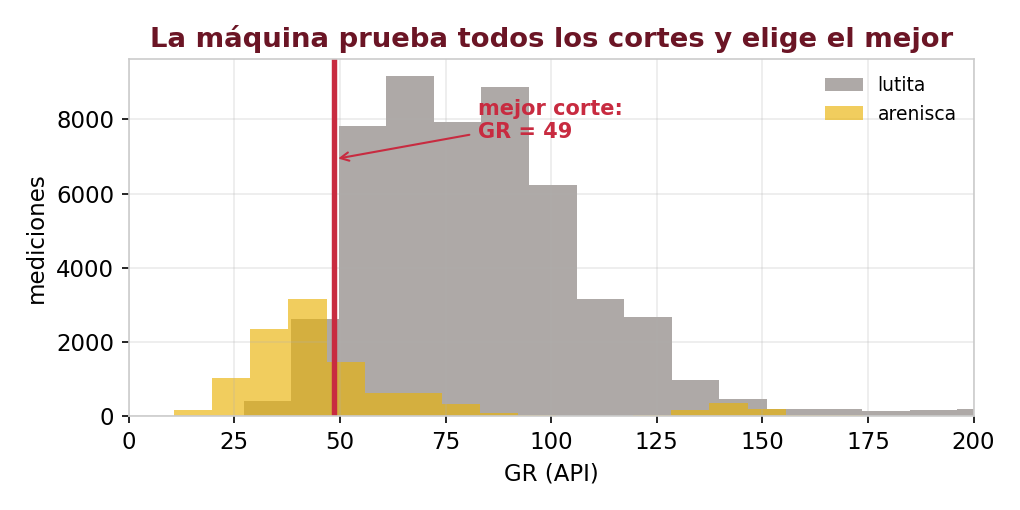
\includegraphics[width=\textwidth]{fig_corte_gr.png}
    \end{column}
    \begin{column}{0.39\textwidth}
      {\footnotesize\color{textMuted}
      \begin{itemize}\setlength{\itemsep}{7pt}
        \item El árbol busca automáticamente un corte de GR.
        \item GR bajo concentra areniscas; GR alto, lutitas.
        \item La zona de traslape exige nuevas preguntas con NPHI, DTC y RHOB.
      \end{itemize}}
      \vspace{5pt}
      {\scriptsize\color{arcaDark}\itshape
        Eso es crecimiento recursivo: resolver primero la división más útil
        y después refinar cada lado.}
    \end{column}
  \end{columns}
\end{frame}

\begin{frame}{Tres Modelos, los Mismos Datos de Prueba}
  \vspace{-6pt}
  \centering
  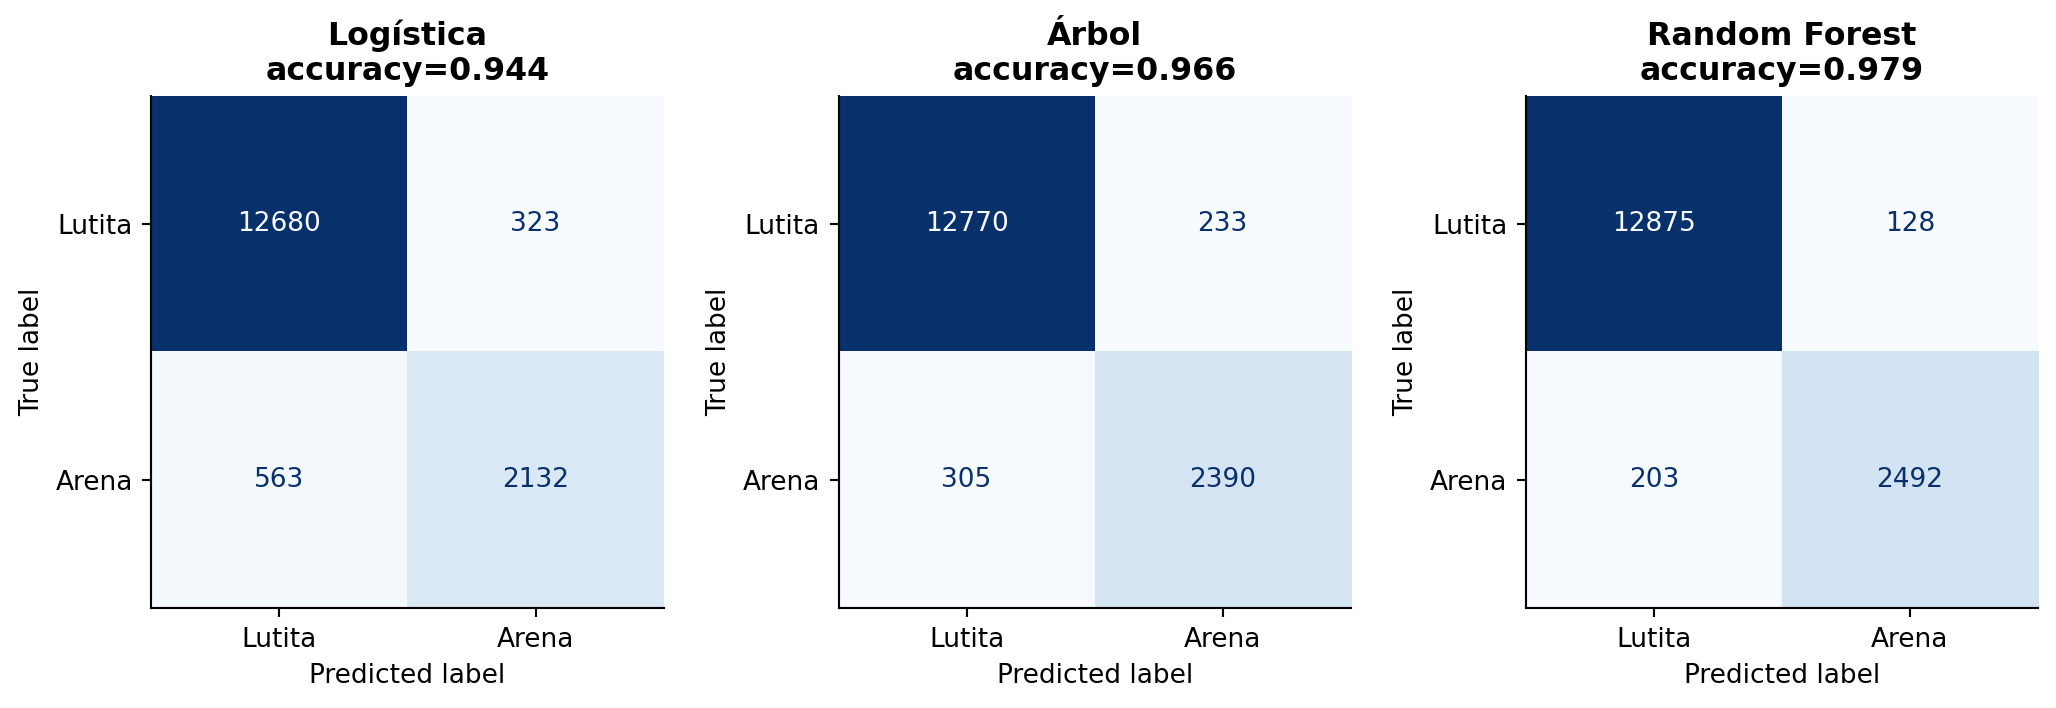
\includegraphics[width=0.96\textwidth,height=0.73\textheight,keepaspectratio]{fig_confusiones_modelos.png}

  \vspace{2pt}
  {\scriptsize\color{textMuted}
    La matriz permite ver dónde mejora: falsos positivos y, especialmente,
    arenas perdidas (falsos negativos). Accuracy sola no cuenta esa historia.}
\end{frame}

\begin{frame}{El Resultado Importante: el Costo Baja}
  \vspace{-6pt}
  \begin{columns}[T]
    \begin{column}{0.56\textwidth}
      \centering
      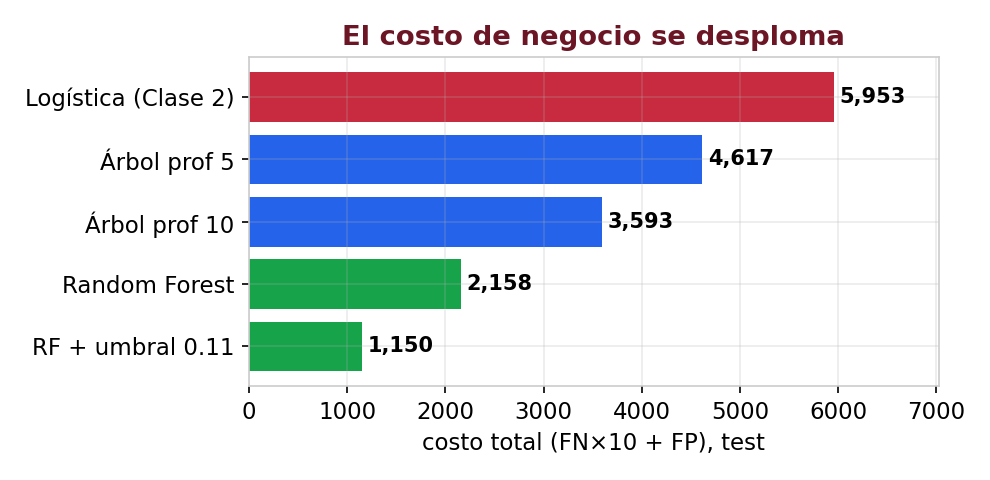
\includegraphics[width=\textwidth]{fig_costo_modelos.png}
    \end{column}
    \begin{column}{0.40\textwidth}
      {\footnotesize\color{textMuted}
      \begin{itemize}\setlength{\itemsep}{7pt}
        \item La logística de la Clase 2 sirve como baseline.
        \item El árbol captura interacciones y reduce arenas perdidas.
        \item El bosque baja el costo de 5\,953 a 2\,158:
          \textbf{64\,\% menos}.
      \end{itemize}}
      \vspace{4pt}
      {\scriptsize\color{arcaDark}\itshape
        Modelo mejor = mejor decisión bajo el costo definido,
        no simplemente mayor accuracy.}
    \end{column}
  \end{columns}
\end{frame}

\begin{frame}[fragile,shrink=12]{El Cambio en Código es Pequeño}
  \vspace{-4pt}
  \begin{columns}[T]
    \begin{column}{0.53\textwidth}
      \begin{pyblock}
from sklearn.ensemble import RandomForestClassifier

rf = RandomForestClassifier(
    n_estimators=200,
    random_state=42)

rf.fit(X_train, y_train)
proba = rf.predict_proba(X_test)[:, 1]
      \end{pyblock}
    \end{column}
    \begin{column}{0.43\textwidth}
      {\scriptsize\color{textMuted}
      \begin{itemize}\setlength{\itemsep}{6pt}
        \item Sigue entregando probabilidades.
        \item El umbral y la matriz de costos de la Clase 2 siguen vigentes.
        \item No necesita \texttt{StandardScaler}.
        \item Puede mostrar importancia de variables.
      \end{itemize}}
    \end{column}
  \end{columns}
\end{frame}

% ═════════════════════════════════════════════════════════════════════════════
\sectionframe{Cierre}{Lo que se llevan hoy}
% ═════════════════════════════════════════════════════════════════════════════

% ── RECAP ────────────────────────────────────────────────────────────────────
\begin{frame}{Lo Que Aprendimos Hoy}
  \vspace{-6pt}
  \begin{columns}[T]
    \begin{column}{0.48\textwidth}
      {\footnotesize\color{arcaDark}\bfseries Conceptos}
      \vspace{3pt}
      {\footnotesize\color{textMuted}
      \begin{itemize}\setlength{\itemsep}{2pt}
        \item[{\color{codeGreen}\scriptsize\faCheck}]
          No linealidad: el paso deja de ser parejo
        \item[{\color{codeGreen}\scriptsize\faCheck}]
          La recta/logística fracasan (las lunas)
        \item[{\color{codeGreen}\scriptsize\faCheck}]
          Árbol = cascada de cutoffs \textbf{aprendidos}
        \item[{\color{codeGreen}\scriptsize\faCheck}]
          \texttt{max\_depth} y el overfitting visible
        \item[{\color{codeGreen}\scriptsize\faCheck}]
          Random Forest: promedio de muchos árboles
        \item[{\color{codeGreen}\scriptsize\faCheck}]
          Importancia de variables (\(\neq\) causalidad)
        \item[{\color{codeGreen}\scriptsize\faCheck}]
          El trade-off poder vs explicabilidad
      \end{itemize}
      }
    \end{column}
    \begin{column}{0.48\textwidth}
      {\footnotesize\color{arcaDark}\bfseries Herramientas}
      \vspace{3pt}
      {\footnotesize\color{textMuted}
      \begin{itemize}\setlength{\itemsep}{2pt}
        \item[{\color{arcaRed}\scriptsize\faTools}]
          \texttt{DecisionTreeRegressor} / \texttt{Classifier}
        \item[{\color{arcaRed}\scriptsize\faTools}]
          \texttt{RandomForestRegressor} / \texttt{Classifier}
        \item[{\color{arcaRed}\scriptsize\faTools}]
          \texttt{plot\_tree}, \texttt{feature\_importances\_}
        \item[{\color{arcaRed}\scriptsize\faTools}]
          \texttt{max\_depth}, \texttt{n\_estimators}
      \end{itemize}
      }
      \vspace{8pt}
      \begin{tcolorbox}[colback=arcaGray, colframe=arcaRed, boxrule=0pt, leftrule=3pt,
        arc=3pt, left=6pt, right=6pt, top=5pt, bottom=5pt]
        {\scriptsize\color{arcaDark}\bfseries La idea para llevarse:}\\[3pt]
        {\scriptsize\color{textMuted}
          la física de producción es curva. Cuando la recta
          se queda corta, los árboles la capturan ---
          y el bosque la captura \textbf{sin memorizar}.}
      \end{tcolorbox}
    \end{column}
  \end{columns}
\end{frame}

% ── PRÓXIMA ──────────────────────────────────────────────────────────────────
\begin{frame}{Lo Que Sigue}
  \vspace{-6pt}
  {\small\color{arcaDark}\bfseries
    Ya tienen modelos lineales y no lineales. Falta afinar cómo los validamos y ajustamos.}

  \vspace{10pt}
  {\footnotesize
  \begin{itemize}\setlength{\itemsep}{7pt}
    \item[{\color{arcaRed}\Large\faArrowCircleRight}]
      \textbf{Validación seria} --- validación cruzada, y el detalle que dejamos
      anotado: evaluar con \textbf{pozos completos} por fuera.

    \item[{\color{arcaRed}\Large\faArrowCircleRight}]
      \textbf{Afinar las perillas} --- búsqueda sistemática de hiperparámetros
      (\texttt{max\_depth}, \texttt{n\_estimators}\ldots).

    \item[{\color{arcaRed}\Large\faArrowCircleRight}]
      \textbf{Multiclase} --- las 11 litologías reales del FORCE 2020, con
      su matriz de penalización de la competencia.
  \end{itemize}
  }

  \vspace{10pt}
  \centering
  {\footnotesize\color{arcaDark}\itshape
    La pregunta de siempre sigue mandando: ¿qué decisión habilita este modelo
    y cuánto cuesta equivocarse?}
\end{frame}

% ── GRACIAS ──────────────────────────────────────────────────────────────────
\begingroup
\setbeamertemplate{headline}{}
\setbeamertemplate{footline}{}
\setbeamertemplate{navigation symbols}{}
\begin{frame}[plain, noframenumbering]
  \begin{tikzpicture}[remember picture, overlay]
    \fill[arcaDark] (current page.south west) rectangle (current page.north east);
    \node[anchor=center, text=white, font=\Huge\bfseries]
      at ([yshift=1.5cm]current page.center) {¡Gracias!};
    \node[anchor=center, text=white!80, font=\large, text width=10cm, align=center]
      at ([yshift=0.2cm]current page.center)
      {Carlos Enrique Mosquera Trujillo};
    \node[anchor=center, text=white!60, font=\normalsize, text width=10cm, align=center]
      at ([yshift=-0.6cm]current page.center)
      {\faEnvelope\hspace{6pt}cmosquerat@unal.edu.co};
    \node[anchor=center, text=white!60, font=\normalsize, text width=11cm, align=center]
      at ([yshift=-1.3cm]current page.center)
      {Machine Learning for Petroleum Engineers Using Python};
    \node[anchor=center, text=white!40, font=\small]
      at ([yshift=-2.0cm]current page.center)
      {SLB Ecuador \quad$\cdot$\quad UDLA \quad$\cdot$\quad 2026};
  \end{tikzpicture}
\end{frame}
\endgroup

\end{document}
